\iffalse

szöveget végignézni, további hivatkozásokat beszúrni

------------------------------------------

Lokalizált:

hivatkozásokat, kiegészítéseket a Tanulmány részbe
--dev-mode és --zero-mode kifejtése
service és embedded mód
JPA jobb kifejtése
migrációs rendszer ötletének kifejtése (ez egyébként diplomamunkának is jó lehet)

------------------------------------------

algoritmusok rendbetétele

mérések: JMH stb.
LargeInteger méréseinek és indokainak részletezése
SQL-mérések
integrált mérések
egyéb mérések (permutációk)
quality mutatók

(kérdőív? legalább írni róla, mint következő lépésről)

\fi



\documentclass[
    parspace,
    noindent,
    nohyp,
]{elteiktdk}[2023/04/10]

\usepackage[dvipsnames]{xcolor}
\usepackage{colortbl}
\usepackage{graphicx}
\usepackage{svg}
\usepackage{hyperref}
\usepackage{cleveref}
\usepackage{appendix}
\usepackage{float}
\usepackage{pgfplots}
\usepackage{arydshln}
\usepackage{fontawesome}
\usepackage{picture,xcolor}
\usepackage{pdflscape}
\usepackage{fancyvrb}
\usepackage{algorithm}
\usepackage[rightComments=false,italicComments=false,breakable=true]{algpseudocodex}
\usepackage[backend=bibtex,style=numeric]{biblatex}
\usepackage[newfloat]{minted}
\usepackage{todonotes}
\usepackage{tocloft}
\renewcommand{\cftsecfont}{\small} % Section titles in smaller font
\renewcommand{\cftsubsecfont}{\small} % Subsection titles in smaller font
\renewcommand{\cftsecpagefont}{\small} % Page numbers in smaller font
\setlength{\cftbeforesecskip}{-0.15em} % Adjust spacing between section entries
\setlength{\cftbeforesubsecskip}{-0.15em} % Adjust spacing between subsection entries

\newcommand{\rhpad}{\vspace{0.6\baselineskip}}


\newcommand{\thesispar}[1]{
\vspace{1em}
\hspace{0.7cm}\parbox[left][][c]{15.8cm}{\linespread{1.2}\selectfont #1}
\vspace{1em}
}


\definecolor{lightyellow}{RGB}{255, 245, 215}
\definecolor{verylightgray}{rgb}{0.96,0.96,0.96}

\newcommand{\todoref}[1]{\todo[inline, noinlinepar, color=red, textcolor=white, inlinewidth=0.6cm, caption={#1}]{\large \textbf{×}}}

\newcommand{\algorithmref}[1]{\hyperref[algorithm:#1]{\colorbox{lightyellow}{%
(\textrightarrow~Algoritmus: \nameref*{algorithm:#1})}}}

\newcommand{\regextt}[1]{\texttt{\colorbox{verylightgray}{#1}}}


\title{HoloDB: Relációs demóadatok on-the-fly generálása deklaratív konfigurációból}
\date{2024}
\author{Horváth Dávid \\ {\small\href{mailto:horvathdown@student.elte.hu}{horvathdown@student.elte.hu}} }
\degree{Programtervező Informatikus BSc}

\supervisor{Dr. Vincellér Zoltán}
\affiliation{Mesteroktató}

\university{Eötvös Loránd Tudományegyetem}
\faculty{Informatikai Kar}
\department{Információs Rendszerek Tanszék}
\city{Budapest}
\logo{elte_cimer_szines}

\addbibresource{references.bib}

\setcounter{tocdepth}{2}
\setcounter{secnumdepth}{2}

\begin{document}

\documentlang{hungarian}

\listoftodos
\cleardoublepage

\maketitle

\begin{small}
\tableofcontents
\end{small}
\cleardoublepage


\begin{abstract}
A modern szoftverfejlesztési módszertanok fő fókuszai közé tartozik
a gyors prototípusgyártás és a (kézi illetve automatizált) integrált tesztelés.
Mindkét esetben tesztadatokat kell biztosítanunk az alkalmazás működtetéséhez.
Ugyanakkor általában demóadatokra számos egyéb helyzetben is szükségünk lehet
(például mockolás, füst-teszt, szoftverbemutató, edukáció).
Nem csak a demóadatok előállítása (jellemzően generálás vagy anonimizálás)
jelent folyamatos terhelést a fejlesztési infrastruktúrára,
de azok indítási, működtetési és memóriaigénye is jelentős, hiszen hús-vér adatbázisokról van szó.
A pályamunkában egy jelentősen újszerű megközelítést mutatok be,
mely szükségtelenné teszi az adatok előzetes előállítását.
A HoloDB egy (felhasználói szemszögből szokványos) relációs adatbázis,
mely minimális indulási idővel és memóriaigénnyel futtatható
egy deklaratív konfigurációs fájlból, mely tömören leírja az adatbázis szerkezetét
és az adataival szembeni követelményeket.
Az on-the-fly generálás miatt maguk az adatok nem foglalnak memóriát,
ugyanakkor a szerver egy lekérések között is koherens adathalmazt szolgáltat.
Számos célmegoldás (köztük kriptográfiai módszerek) együttes alkalmazásával
koherens és gyors működést biztosító adatelérési technikák váltak lehetővé (például a virtuális indexek),
így a HoloDB (alkalmas skálázás mellett) runtime performanciában
sem marad alul a hagyományos adatbázisokkal szemben.
A relációs modell a megfelelő adapterekkel könnyen kiterjeszthető más adatmodellekre is
(például NoSQL, GraphQL).
Az új megoldás reményeim szerint további előnyök mellett
ötvözi a korábbi megoldások erősségeit, míg kikerüli azok fő hátrányait.
Valamint olyan új lehetőségek nyílnak meg, mint a „dev mode”
(az adatbázis azonnali frissülése a konfigurációs fájl módosításakor)
vagy a serverless adatbázis-szolgáltatás.
\end{abstract}

\chapter{Bevezetés}

\section{Problémafelvetés}

A szoftverfejlesztési és -release-elési folyamatok lényeges előfeltevése,
hogy az alkalmazás mint absztrakt entitás snapshot jellegű,
azaz a mindenkori forráskód \textit{aktuális állapotának} derivátuma,
nem függ annak történetiségétől.
Ezt az átlátható képet bolygatja meg a szoftverhez tartozó produkciós adatbázis,
mely önálló életet él, a felhasználói világgal való interakcióban folyamatosan változik;
szerkezete, szemantikája azonban szorosan az alkalmazás mindenkori állapotához kötődik.%
\cite{Ploski2007DatabaseCentricVersioning,Fluri2023DatabaseCiCd,Edwards2023LiveLocalSchemaChange}

Az \textit{életnek kitett} produkciós adatbázist természetesen kénytelenek vagyunk
minden erőforrásigényével életben tartani, és minden release-zel migrálni \todoref{+CITE: DB-migráció (Flyway/Liquibase...?)}.
Ám az \textit{absztrakt értelemben vett} adatbázisra számos egyéb helyen is szükségünk van,
ahol ezek a folyamatos költségek igencsak nemkívánatosak.
Ilyenek esetek jellemzően az integrációs és egyéb tesztelés, gyors prototípusgyártás, kísérletezés draft adatbázisokkal, rövid demonstrációk és prezentációk.

Mivel más opció fel sem merül, ezekben az esetekben is ugyanahhoz az infrastruktúrához nyúlunk,
mint a produkciós adatbázis esetében.
Így például az integrációs tesztek is jelentős erőforrást fognak igénybe venni
(generálási vagy anonimizálási időt, indítási  és üzemeltetési költséget, memória- és tárhelyfoglalást stb.),
mindezt egy rövidéletű adathalmaz biztosítása miatt,
amelynek ráadásul csak töredéke lesz érintve egy-egy teszt során.

Gyakran tehát szükségünk van egy működő adatbázisra,
miközben valójában nincs szükségünk igazi adatokra.
Meglehetősen paradox ez a helyzet.
Ráadásul van valami abszurd abban, amikor ilyen nagy mennyiségű adatot
gondosan lematerializálunk, hogy aztán nagyrészt használatlanul eldobjuk.
Még ha olykor fel is merül a kérdés, hogy vajon elkerülhető-e mindez,
más egyértelmű megoldás híján továbbra is inkább a meglévő módszerek tökéletesítésére törekszünk.
Ördögi kör.

Amikor egy szoftver kezdeti fázisában az adatbázis szerkezete is gyakran változik,
a próbálgatáshoz, teszteléshez fenntartott lokális adatbázist folyton újra létre kell hozni,
vagy pedig igazítani a megváltozott adatszerkezethez.
Mindkét megközelítés nehézségekkel és erőforráshasználattal jár.
Sokkal egyszerűbb lenne az adatbázis szerkezetét egyetlen deklaratív konfigurációs fájltól
(vagy akár közvetlenül az alkalmazásban definiált adatosztályok szerkezetétől) függővé tenni.

A dolgozatban elsősorban ezekre a problémákra kínálok egy újszerű megoldást.
Mivel a bemutatott szoftver egyúttal egy általános keretrendszer virtuális adattárakhoz,
számos további alkalmazása is adódhat.

\section{Tanulmány}

\subsection{A probléma státusza}

Érdemes tisztázni, hogy nem ismerek még csak próbálkozást sem,
mely a fenti problémafelvetésemre kívánt volna célzott megoldást találni,
és főképpen nem tudok olyanról, amely ilyesmit már nyújtana.
Természetesen valaminek a hiányát nehéz bizonyítani,
és az állítást (egyelőre) pusztán egy sokéves fejlesztői tapasztalat
során szerzett erőteljes benyomás támasztja alá.

Számomra meglepő, hogy egy ilyen nehézségre,
mely napi szinten érinti fejlesztők, tesztelők és mások munkáját, produktivitását,
egyelőre csak a legszofisztikáltabb \textit{kerülőmegoldások} születtek.
Hamarosan megkísérlem megtippelni ennek az okát.
Előbb azonban röviden áttekintem azokat a tipikus megoldásokat,
melyek valamennyire kapcsolódnak ehhez a problémához,
némileg hasonlót akarnak megoldani.

\subsection{Kérések mockolása on-the-fly}

Főként webes API-k által szolgáltatott adathalmazok mockolásakor találkozunk olyan megoldással,
mely a lekérés (és persze az előre beállított szabályok)
alapján generálja a válaszként visszaadandó adatstruktúrát
(például egy rekordot vagy dokumentumot JSON formátumban).
Az adatok véletlenszerűen kerülnek kitöltésre a lekérés szerkezete alapján megállapított séma keretébe.
\todoref{+CITE: API-mockolók}

A módszer SQL-lekérdezések közvetlen mockolásához is adaptálható,
a lekérdezés (és ha ismert, akkor a séma) alapján meg kell állapítani
a visszaadandó eredménytábla szerkezetét, adattípusait,
az egy-egy oszlopba kerülő adatok jellegét,
majd random jelleggel elő kell állítani bizonyos számú, ezeknek a követelményeknek megfelelő eredményrekordot.
\todoref{+CITE: SQL-mockolók}

Ebbe a kategóriába sorolhatók az úgynevezett faker segédkönyvtárak is.
Ezek olyan véletlenadat-generálók,
melyek bizonyos gyakori entitástípusok adatait (pl. személynevek, e-mail, dátum) szolgáltatják.
\todoref{+CITE: faker segédkönyvtárak}

Ez a megközelítés természetesen nem is törekszik arra,
hogy koherens eredményt adjon több lekérés esetén,
tehát csak olyankor használható, ahol a lekérések nem épülnek egymásra.
Cserébe erőforrásigénye csekély, nincs szükség az adatok tényleges tárolására.
\todoref{kérések mockolása: az on-demand schema ennek a koherenssé tett változata is}

\subsection{Seed-alapú virtuális világok}

Játékokban és egyszerűbb szimulációkban már igen régóta generálnak kisebb világokat,
pályákat procedurálisan valamilyen pszeudovéletlen algoritmus segítségével.
Ennek azonban komoly méretbeli korlátai vannak.
Felmerül a gondolat, hogy lehetséges-e óriás méretű világokat konzisztensen
a játékosok rendelkezésére bocsátani, anélkül, hogy le kellene generálni az egészet.

Univerzumot, nyílt világokat és egyéb óriás rendszereket felvonultató játékokban
a probléma már régen felmerült, és természetesen megoldások is születtek.
Egy ilyen módszer, ha a világteret (sorosan vagy hierarchikusan)
szeletekre osztjuk, és biztosítunk egy függvényt,
mely minden szelethez rendel egy saját seed értéket.
Legegyszerűbb esetben a seed az adott szelet sorszámából generált hash.
Amikor szükségünk van valamely szelet tartalmára, a szelet seedjéből kiindulva,
az adott szabályrendszer szerint on-demand legeneráljuk az adott szelet tartalmát.
A sűrűn benépesített világok szomszédos szeleteinek összeillesztése néha nem triviális.
Felületszerű, folytonos struktúrák generálása esetén gyakran használnak
valamilyen eleve interpolált eljárást,
így biztosítva a töretlen átmenetet a szomszédos szeletek határvonalainál.

Egy közismert korai példa seed-alapú módszert alkalmazó szoftverre
az \textit{Elite} nevű 1984-ben kiadott űrhajós videójáték
\todoref{+CITE: Játék: Elite (1984)}.
A játékban meglátogatható bolygók kapnak egy-egy seedet, mely már teljesen determinálja a felépítésüket,
így elég a bolygó meglátogatásakor legenerálni a tartalmát.
A módszert aztán átvették és továbbfejlesztették az újabb és újabb óriástérképes játékok.
A seed-alapú módszernél valójában nincs határa, mekkora virtuális világot definiálhatunk.
Az Elite sikere után hamar megjelent a kifejezetten végtelen nyílt világ koncepciója,
mely meghatározó eleme olyan közismert játékoknak,
mint a \textit{Starflight} (1986) \todoref{+CITE: Játék: Starflight (1986)},
a \textit{Minecraft} (2011) \todoref{+CITE: Játék: Minecraft (2011)},
a \textit{Starmade} (2012) \todoref{+CITE: Játék: Starmade (2012)},
a \textit{No Man's Sky} (2016) \todoref{+CITE: Játék: No Man's Sky (2016)},
a \textit{Starfield} (2023) \todoref{+CITE: Játék: Starfield (2023)}~
stb.

Ha elvonatkoztatunk a játékoktól és szimulációktól,
ez a generálási módszer közel tetszőleges jellegű virtuális adathalmaz böngészését képes biztosítani.
De azonnal szembeötlik a legfőbb hátrány is: a virtuális világ-adathalmaz nem kereshető.
Nem tudjuk például hatékonyan lekérdezni, mely világszeletekben lelhető föl egy adott típusú objektum.

\subsection{Relációs adatok generálása}

Amikor adatokat generálunk egy relációs modellbe, azt legegyszerűbb megközelítésben fölfoghatjuk úgy is,
mint az előbb bemutatott virtuális világ materializációját egy relációs adatbázisszerveren.
Milyen előnyöket nyerünk ezzel? Lássunk néhányat:

\begin{itemize}
    \item utófeldolgozás: utólag holisztikus módosításokat eszközölhetünk az adathalmazon
    \item egynemű módosíthatóság: minden eleve tárolva van, nem kell külön kezelni a változásokat
    \item kereshetőség: az adatbázis-kezelő biztosítja az indexeket
\end{itemize}

A fő hátrány egyértelmű: a nagy tárhelyigény.
Vegyük észre, hogy még a kereshetőség is az indexek által foglalt további tárhely által valósul meg
(az adatok eleve nagy tárhelyfoglalása mellett tűnhet esetleg elhanyagolhatónak).
Ha pedig nem materializált adatok mellé gyártunk indexeket,
akkor ki kell dolgoznunk valamilyen módszert a módosulások detektálására, ami általában nem triviális.

Egyes generátorok a séma és az adatok jellegének deklaratív leírását is támogatják. Ez a leírás tárolható egy konfigurációs fájlban, ami verziókezelhető, dokumentálható, könnyen szerkeszthető.
\todoref{+CITE: DB deklaratív adatgenerátorok}

\subsection{Relációs adatok anonimizálása}

Ha már rendelkezésre áll egy éles adatbázis, kézenfekvőnek látszik,
hogy ennek replikáit használjuk a teszt- vagy mockadatbázis kiindulópontjaként \todoref{+CITE: DB-anonimizálók}.
Így rögtön egy valószerű adathalmazzal indulunk,
az érzékeny adatok miatt azonban anonimizálásra van szükség.
Tehát a generáláshoz szükséges számítási igényt összességében
felcseréljük a másolás és anonimizáció költségeivel.

Úgy tűnik, gyakran anonimizálással együtt is egyszerűbb dolog meglévő adatokból kiindulni,
mint egy komplett generálási folyamatot kiépíteni.
Egy köztes megoldás lehet a séma és az adatok nagyjábóli jellegének letapogatása,
és az ez alapján történő újragenerálás.

Azonban a bevezetőben felsorolt szituációk egy részében
nem is áll rendelkezésre egy létező produkciós adatbázis.
És ha rendelkezésre is áll, további probléma,
hogy az adatok megszerzéséhez az éles adatbázist kell felkeresni,
ami egyfelől az éles környezet nemkívánatos terhelését jelenti,
másrészt az oda való beauthentikálás (a konkrét megoldástól függően) biztonsági kockázatot rejthet.

Egy általános megoldás tehát aligha épülhet anonimizálásos módszerre.

\subsection{Nagy teljesítményű megoldások}

Számos nagyteljesítményű szolgáltatás érhető el a piacon szintetikus adatok generálásához.
A \textit{MOSTLY AI} megoldása az akkurátus adatokra helyezi a hangsúlyt.
Az adatok statisztikai jellemzői és mintázatának lényeges elemei
jól illeszkednek a valós adatoknál látható mintázatokra. \todoref{+CITE: Nagy teljesítményű megoldás: MOSTLY AI}

Egyes platformok általános megoldást nyújtanak az adatgenerálásra, anonimizációra és CI/CD-integrációra.
Ilyen például a \textit{Tonic}, a \textit{GenRocket} és a \textit{Delphix}. \todoref{+CITE: További nagy teljesítményű megoldások: Tonic, GenRocket, Delphix}

Ezek a rendszerek erősen optimalizálják és párhuzamosítják a tesztadatok előállításának egyes lépéseit,
így a fapados megoldásokhoz képest költséghatékonyak.
Csodát viszont nem lehet várni: a számításigény aszimptotikusan,
a tárhelyigény pedig teljes egészében ugyanaz marad.

\subsection{Miért csak kerülő megoldások vannak?}

A rohanó világban, különösen a lokális optimumra törekvő fejlesztők világában,
az egyértelmű alternatív megoldás hiánya szükségszerűen
a bevett kerékvonalak továbbmélyítését eredményezi.
Úgy látszik, hogy egy újszerű megoldással való kísérletezés egyszerűen
kívül esik a megszokott paradigmán, és nem fér bele az időbe.

Néhány ezzel kapcsolatos tényezőt tényszerűen megállapíthatunk.

\begin{itemize}
    \item \textbf{Érdekhiány}: a releváns területen működő nagyobb vendorok elsősorban
          erőforrásokat adnak bérbe, és az általuk fejlesztett architektúrák (történetileg érthetően)
          elsősorban az ezeken futó tényleges adatbázisok kezelését kell megoldják;
          nincs tehát nyomás jelentősen más típusú termékkel való kísérletezésre.
          \todoref{+CITE: (miért nincs?) erőforrásokat adnak bérbe}
    \item \textbf{Bejáratott alternatívák}: az on-the-fly mockolás lehetősége,
          a NoSQL adatbázisok és felhőmegoldások fejlődése stb.
          sztenderdképző kerülőmegoldásokként elfedték a problémát.
          \todoref{+CITE: (miért nincs?) kerülőmegoldások}
    \item \textbf{Megfelelő SQL plannerek eddigi hiánya}: az Apache Calcite például
          csak az utóbbi néhány évben vált népszerűvé, és inkább elsősorban adatintegrátorként.
          \todoref{+CITE: (miért nincs?) SQL-plannerek csak utóbb}
    \item \textbf{Kontraintuitivitás}: az új megoldás működésmódja nem triviális,
          így nem egyszerű átlátni a koncepciót, és megérteni hogy „hol is vannak az adatok”.
          \todoref{+CITE: (miért nincs?) hol is vannak az adatok}
\end{itemize}

Jelenleg csak tippelni tudok, mennyire okozói ezek (illetve ezek összjátéka) a vizsgált helyzetnek.
Érdemes lenne ezt a kérdést a későbbiekben külön tanulmányban alaposabban is megvizsgálni,
nagyban építve egy megfelelően megtervezett, fejlesztőkre és technikai vezetőkre is kiterjedő kérdőíves kutatásra.

\section{Az új megközelítés}

A következőkben lényegileg egy sajátos relációsadatbázis-szervert fogok bemutatni.
Ennek a már működő és kipróbálható szoftvernek a HoloDB nevet adtam.
Kezdetben ugyanis úgy gondoltam rá,
mint a hologram-ábrák megfelelőjére az adatbázisok világában,
mint ami illuzórikusan kerül kivetítésre egy kis méretű definícióból.
Ebben az adatbázisban ugyanis nincsenek tárolva adatok
(legfeljebb adatok változásai, ha az írhatóság be van kapcsolva).

A deklaratív konfiguráció alapján a lekérdezések eredménye on-the-fly kerül kiszámításra,
úgy, hogy a lekérdezések közötti konzisztencia biztosított,
vagyis az egymás utáni lekérdezések egy koherens adatbázis képét adják.
Ezt pusztán adatmezőnként determinisztikusan generált értékekkel is meg lehetne oldani,
ekkor a kereséshez a teljes tábla szkennelése lenne szükséges
(vagyis visszajutnánk ugyanahhoz a problémához,
mint amit a seed-alapú világokban való kereshetőség kapcsán említettem).
A virtuális indexeknek köszönhetően azonban nincs szükség ilyen költséges műveletekre.
Az értéklekérés és keresés oda-vissza egybecsengő működésének
biztosításához a kriptográfiából ismert módszereket is felhasználtam.

A végeredmény egy skálázható és testreszabható nyílt-forráskódú adatbázis-mockoló eszköz,
számos kiegészítővel
(REPL; networking; JDBC és JPA támogatása, Docker, haladó értékkészletek stb.).

Mivel nincsenek adatok, a memóriafogyasztás minimális,
különösen, ha nem érkezik egyszerre sok lekérés.
A nem létező adatok természetesen a háttértáron sem foglalnak helyet.
Mivel a szerver elindulása pusztán a konfiguráció betöltéséből áll,
az indulási idő is minimális.
Az egyetlen előzetes költség, amit a felhasználónak be kell fektetnie,
az a konfigurációs fájl megírása,
bár példafájlokból kiindulva ez szinte néhány másolással is megoldható,
illetve akár generálható is.

Az architektúra tárgyalása során kifejezetten a relációs storage API implementációja lesz a fókuszban.
Ez az a szűk keresztmetszet, amely a megoldás újszerűségéhez leginkább hozzájárul,
és ami a prototípusban is a legkidolgozottabb rész.
A forráskód az itt bemutatottakon túl is sok érdekességet rejt,
ezért jó szívvel ajánlom a szoftver Git-tárolóját,
melyet a dolgozat legvégén linkeltem is.

A szoftver \textbf{Java környezetben készült},
a továbbiakban ez implicite odaértendő akkor is,
ha külön nem hívom fel rá a figyelmet.

\section{Alkalmazhatóság}

A fentiek fényében az alábbi területeken biztosan alkalmazható a szoftver:

\begin{itemize}
    \setlength\itemsep{-0.4em}
    \item \textbf{Tesztelés:} Integrációs és egyéb tesztek, kipróbálás.
    \item \textbf{Fejlesztés:} Kezdeti fázisban, prototípusoknál, gyakran változó adatszerkezet esetében.
    \item \textbf{Demonstrációk:} Példaadatok szolgáltatásához bemutatókhoz, koncepciótervekhez.
    \item \textbf{Oktatás:} Ad hoc adathalmaz biztosításához konkrét példákhoz és feladatokhoz.
\end{itemize}

Mivel az új megoldás erőforrásigénybeli paraméterei
radikálisan eltérnek a tényleges adatbázisokétól,
számos olyan helyen is felmerülhet az alkalmazása,
ahol hagyományosan rossz gyakorlatnak számít adatbázisszervert futtatni.
Ilyen esetek például: füsttesztek, unit tesztek, serverless.

Néhány olyan lehetőség is megnyílik, ami adatbázisok esetében eddig fel sem merült.
Ilyen például a \textbf{dev mode}, amikor a konfiguráció módosításával a teljes adatbázis
azonnal igazodik a módosításhoz. \todoref{dev-mode, zero-mode (az on-demand schema részt is ehhez igazítani)}

\section{Célkitűzések}

A következőket fogjuk elvárni a megoldástól:

\begin{enumerate}
    \setlength\itemsep{-1em}
    \item Támogatja a relációs adatmodellt.
    \item Determinisztikus, koherens.
    \item Az adatok könnyen variálhatóak.
    \item Óriás adatmennyiséget is képes szimulálni.
    \item Gyors, indexelt keresést nyújt, a lekérések időigénye elfogadható.
    \item Azonnal elindul, nincs számottevő preparálási folyamat.
    \item Kevés memóriát foglal, az adatokat on-the-fly számítja.
    \item Könnyen és rugalmasan konfigurálható.
    \item Skálázható, finomhangolható.
    \item Egyedi működéssel könnyen bővíthető.
    \item Opcionálisan írható.
\end{enumerate}

\section{Megjegyzés a dolgozat koncepciójához}

A dolgozat egy újszerű megoldást mutat be a fentebb megfogalmazott problémára.
Fő célja az elképzelés működőképességének bizonyítása,
tehát annak a láncnak a bemutatása,
mely a különféle részmegoldásokat egybefűzi,
hogy létrehozza a relációs adatbázis illúzióját,
miközben megfelel ez imént megfogalmazott célkitűzéseknek.
Mind a fejlesztés, mind a dolgozat írása során
a szoftvertechnológiai és architekturális szempontokra koncentráltam.
A későbbiekben természetesen egyre fontosabbá válik majd az implementációs lehetőségek
részletes analízise, nagy mennyiségű mérési adat felhalmozása és összehasonlítása.
Ha azonban kezdettől ezekre az aspektusokra koncentráltam volna,
lehetetlen lett volna egy ilyen átfogó koncepció megvalósítása és bemutatása.
Így a felvonultatott mérési eredmények is kifejezetten azt a célt szolgálják,
hogy az átfogó működőképességet integrált tesztekből származó számszerű adatokkal alátámasszák.
Figyelembe kell venni azt is,
hogy a projekt nem egy már bejáratott nagyobb kutatási program része,
egyelőre nincsenek további dedikált erőforrásai
a részterületek mérési adatainak feldolgozására.
\todoref{+CITE: a dolgozat koncepciója: a mérések fényében ezen enyhíteni}


\chapter{Architektúra}

\section{A nagy illúzió: adatok a semmiből}

Olyan adatszolgáltatás felépítésére vállalkozunk tehát,
mely egy \textbf{tetszőlegesen nagy méretű, koherens és kereshető} adattárat imitál,
miközben mindebből semmi sem létezik fizikálisan.
Hogy egy koherens adattároló látszatát elérjük,
apró eszközök egész tárát kell összeverbuválni,
akár olyan távol eső területekről mint az automataelmélet és a kriptográfia.
Mivel a cél egy felhasználói szemszögből is áttekinthető és rugalmas eszköz biztosítása,
választanunk kell egy kellően általános adathozzáférési modellt a virtuális adathalmaz prezentálásához.
Ez az adatmodell a relációs adatmodell lesz,
melyhez egy konkrét \textbf{relációs storage API}-t fogunk definiálni.
Aligha érdemes más megközelítést választani,
hiszen a relációs adatmodell nem csak tradicionálisan megkerülhetetlen
és máig a legnépszerűbb adattárolási módszer\cite{DBEngines2024RankingModels},
de egyúttal egy olyan általános adatelérési normalizációs szabvány,
mely közös nevezőként tud szolgálni további modellhez (például NoSQL, gráfadatbázisok).

A legtöbb szoftver architektúrájában jól elkülöníthető valamilyen
alapvető szerepet betöltő, fokális entitástípus
(például egy könyvtári katalógusban a \textit{könyv}).
Célszerű lehet ilyen entitást esetünkben is meghatározni,
hogy segítse az architektúrában való eligazodást.
Úgy tűnik, a virtuális adattár legalapvetőbb objektuma az \textbf{\textit{értéklista}}.
Az értéklista egyszerű esete valamely egyszerű \textit{értékkészlet},
az API-ban pedig egy-egy \textit{oszlop} értéklistájával fogunk találkozni.

Egy oszlopban azonos típusú adatok gyűjteménye szerepel.
Ezeket az adatokat általában egy adott \textit{értékkészlet}ből válogatjuk össze.
Jó, ha az értékkészlet rendezett, kereshető;
mint majd látjuk, ez az egyszerű megkötés már általában elégséges ahhoz,
hogy maga az oszlop is kereshető legyen.

Néha esetleg ki kell lépnünk a szigorú oszlop-orientáltságból.
Lehetnek például összefüggések egy táblán belüli oszlopok között.
Ezt azonban még mindig egyszerűbb az oszlopos megközelítés megfelelő kiterjesztésével elérni,
mintsem áttérni valamiféle rekordonkénti generálásra.
Úgy is mondhatjuk, hogy az oszlopok alatti mezők jó jelöltek arra, hogy „világszeletek” legyenek,
míg egész rekordok nem.

Lehetnek továbbá megkötések táblák között is.
Ezek kezelése is könnyen elvégezhető az oszlopos alapvetésre építve.
Az egyoszlopos idegen kulcsoknál például csak annyit kell biztosítani,
hogy a hivatkozó oszlop értékkészletét a hivatkozott oszlop tartalma adja.

A mindenkori módszert, amivel egy oszlop értéklistáját biztosítjuk,
\textit{értékkiosztás}nak fogom nevezni.
A virtuális értékkiosztások olyan függvényt valósítanak meg,
mellyel egy adott mező értéke determinisztikusan előállítható.
De az igazán lényeges kihívást az jelenti, hogy szeretnénk,
ha az értéklistában keresni is tudnánk, méghozzá hatékonyan,
hasonlóan ahhoz, mint amikor tényleges adatbázisok esetén
az oszlophoz már generálva van egy index.
A virtuális adattár esetén is lehetséges lenne indexeket generálni,
de ez az adatok materializálásával járna,
a virtuális adattár mégse lenne többé virtuális.
Ideális esetben tehát az indexek is virtuálisak
(ennek oda-vissza koherensnek kell lennie; itt jön majd képbe a kriptográfia).
Elsősorban olyan megoldásokat fogok bemutatni,
amelyek teljesítik a kereshetőség erősebb feltételét is,
azaz \textbf{kereshető virtuális értékkiosztások}.

A legtöbb oszlop értékkészlete jól behatárolható.
Az oszlopban tételesen szereplő értékek egy efölötti
tetszőlegesen sorrendezett multihalmazt (tömböt) alkotnak,
néha ehhez statisztikai megkötések is tartoznak ($NULL$-ok száma, értékgyakoriság stb.).
A tábla rekordjait sorrendezettnek fogom tekinteni:
azonos táblabeli valamely két oszlop értéklistájából kiválasztott egy-egy mező
azonos rekordhoz tartozik pontosan akkor, ha a sorrendbeli pozíciójuk (sorindexük) megegyezik.

Vegyük észre, hogy több független, külön-külön is implementálható problémával szembesülünk:

\begin{enumerate}
    \item az értékkészlet biztosítása
    \item az értékkészlet monoton rendezett multihalmazának képzése
    \item az értékek összekeverése
\end{enumerate}

A multihalmaz itt egy monoton növekvő tömböt jelent,
ezt fogjuk még egy további lépésben összekeverni egy permutáló függvény alkalmazásával.
Ennek a többlépéses módszernek az átláthatóságon kívül az is nagy előnye,
hogy a lépések egymástól függetlenül skálázhatók.

A lépéseket úgy kell megvalósítani, hogy a végső értéklista adott pozíciójú eleme is gyorsan lekérhető legyen,
valamint egy adott érték vagy értéksáv előfordulási pozíciói is
(keresés).
A permutáció esetén ez annyit jelent, hogy legyen effektíve invertálható.

Az értékkészletből történő \textbf{kétlépéses értékkiosztásnak} ezzel az ötletével
egy egyszerűbb adatbázis szimulációjának kívánalmait már tulajdonképpen le is fedtük,
de néhány további hasznos értékkiosztási módszert is be fogok majd mutatni.

Ha oszlopokat elő tudunk állítani,
akkor a táblák és egyéb objektumok köréépítése nem jelent kihívást.
Ha pedig a relációs adatmodell ezen objektumait sikeresen implementáltuk,
a relációs műveletek és \textbf{az SQL lekérdezések megvalósítása már a hagyományos módon történhet}.
Éppen ezért a továbbiakban a lekérdezések problémakörével csak érintőlegesen foglalkozom.
Ma már elérhető néhány nyílt forrású jól felépített SQL query planner framework is,
melyek megkönnyítik egy teljes körű SQL-szerver kiépítését.
Ilyen például az általam használt Apache Calcite.
Ugyanakkor egy saját SQL-futtatót is implementáltam, mely sok esetben gyorsabb fut,
cserébe csak limitált SQL-t támogat.


\section{A prototípusról}

A virtuális adatbázist megvalósító szoftvert HoloDB néven tettem elérhetővé.
Az elnevezés a hologramokra utal:
a konfigurációból leképzett, „kivetített” virtuális adatbázis hasonlóan illuzórikus,
mint a hologramból előhívott térbeli látvány.

A HoloDB sok tekintetben már kinőtte a prototípus státuszt,
hiszen egy nagyívű rétegelt architektúráról van szó,
mely kellően megszilárdult alapvonalakkal rendelkezik a hosszútávú fejlesztéshez.
Ugyanakkor stabil verzióról még nem beszélhetünk;
az implementációs részleteket, valós használati eseteket,
más eszközökkel való integrációt illetően még számos felmérendő, kikísérletezendő dolog adódik.

A szerver Docker konténerként is futtatható, amihez a Docker Hubon biztosítok egy testreszabott képet.
A felhasználói Dockerfile mellé csak a konfigurációs fájlt kell elhelyezni az indításhoz.
A testreszabott kép a kis erőforrásigény miatt serverless végpontként is jól használható.

A HoloDB a MiniBase projektre épül.
Utóbbi egy relációsadatbázis-keretrendszer, mely definiálja a storage API-t,
és annak konkrét implementációjához agnosztikusan viszonyulva
egy komplett adatbázisszervert épít fölé;
beleértve a lekérdezések fordítását és futtatását,
a felhasználói munkamenetek, tranzakciók és változók kezelését,
a runtime sémamódosításokat illetve új táblákat és más felelősségi köröket.
A HoloDB ehhez a storage API virtuális implementációját,
a konfiguráció kezelését
és a megfelelő futtatási környezetet adja hozzá.

A MiniBase közvetlenül biztosít egy SQL-futtató felületet, a MiniConnect API megvalósításával.
A MiniConnect testvérprojekt célja egy egyszerű és egyértelmű adatbázis-elérési API definiálása,
melyet a JDBC nehézkessége motivált.
A MiniConnecthez különféle middleware változatok is elérhetők, például hálózaton keresztül is használható,
illetve letisztultsága miatt könnyen írhatók hozzá dekorátorok, proxyk.
Egy (deb csomagként is elérhető) REPL\todoref{mi az a REPL?} is tartozik hozzá,
mellyel parancssorból tudunk hálózaton keresztül csatlakozni a MiniConnectet támogató tetszőleges adatbázishoz.
Ez egyúttal a HoloDB kipróbálásának legkényelmesebb módja,
számos kényelmi funkciót támogat
(szép kimenet, szintaxiskiemelés, automatikus kiegészítés, parancstörténet stb.).

Az architektúra köré sokféle eszközt fejlesztettem,
melyek a robusztusság eltérő fokain állnak.
Ilyenek például: automatikus REST API, GraphQL adapter, authentikációs proxy, Apache Calcite SQL driver stb.
\todoref{A toolokhoz valami leírást még}

\begin{figure}[H]
\centering
\includesvg[height=0.8\textwidth]{diagram/simplearch}
\caption{A virtuális adatbázis vázlatos architektúrája}
\end{figure}


\section{A relációs storage API}

Ha már körvonalaztuk a relációs adathozzáférés fő entitásait,
ezeket rendre implementálva egy funkcionálisan teljes körű relációs adattárat kapunk.
Az entitások meghatározásakor elsőként a \textit{hozzáférés} szempontjait érdemes átgondolni.
Az írhatóság problémakörével később foglalkozom.

Nyilvánvalóan gondoskodni kell az alapvető hierarchiáról,
erre szolgálnak a \texttt{Schema}, \texttt{Table} és \texttt{Column} típusok.
Egy-egy oszlop elvont tulajdonságait a \texttt{ColumnDefinition} típus fogja össze.
Bár az egyes mezők értékeit általában oszloporientáltan állítjuk elő
(jellemzően az értéklistákat megadó \texttt{Source} objektumok használatával),
a lekérések szemszögéből jobbnak mutatkozik a rekordorientált megközelítés.
A rekordot a \textt{Row} típus reprezentálja,
ezen keresztül kérhetőek le a konkrét mezőértékek
az oszlopnév vagy oszloppozíció megadásával.

Az adatok hatékony keresését virtuális indexek fogják segíteni.
Három ilyen indexfajtával fogok foglalkozni:
a normál \texttt{TableIndex}, a \texttt{FulltextIndex} és a \texttt{SpatialIndex} típusokkal.
Ezek keresőmetódusai egy \texttt{TableSelection} példánnyal térnek vissza,
melyen keresztül a találati listához férünk hozzá.
A \texttt{TableIndex} a szokásos rendezett indextípus,
mely egyúttal teljes kontrollal rendelkezik a találati lista rendezése
és a $NULL$ értékek kezelése fölött.
Ha többoszlopos, akkor az oszloplista bármely prefixére is indexként működik (leftmost prefix lookup\todoref{Leftmost prefix lookup: valamit róla}).
A másik két típus találatainak rendezése definiálatlan.
Egyik sem ad vissza $NULL$ mezőket.

A következő osztálydiagramon a vázlatosan összefoglaltam az interfészeket:
\todoref{A possibleValues egy Optional<Source>-szel is visszatérhetne}

\begin{figure}[H]
\centering
\includegraphics[width=0.85\textwidth]{diagram/storage-api-uml.png}
\caption{A storage API fő interfészei (egy relációs adattár alapentitásai)}
\end{figure}


\section{Az írhatósági réteg}

A virtuális adattár egy-egy példánya várhatóan viszonylag rövid élettartamú lesz.
Feltehetjük, hogy az írási műveletek összességében kevés módosítást eredményeznek.
A tipikus szcenáriókban főként egyes konkrét rekordok lesznek módosítva, hozzáadva, törölve.
A tömeges módosítások kérdésével itt nem foglalkozom,
de nem látszik akadálya az ezek optimalizálását célzó továbbfejlesztésnek.

Az írhatósági réteget arra is használhatjuk,
hogy egy-egy tesztesethez egyéni rekordokat adjunk hozzá,
ami megkötéseken keresztül nehézkesebb lenne.

A módosítások támogatásához előszöris a \texttt{Table} interfészt magát
ki kell egészíteni a megfelelő műveletekkel
(pl. \texttt{isWritable()}, \texttt{applyPatch(TablePatch)}, \texttt{sequence()}).
A csak-írható implementáció persze az írási műveleteket nem fogja támogatni.

A \texttt{DiffTable} egy tetszőleges \texttt{Table} implementáció fölé elhelyezhető dekorátor.
Teljesen áttetszően működik: amíg nincsenek módosítások,
minden műveletet egyszerűen továbbít a dekorált tábla felé.
Módosítás esetén a különbségeket (módosított értékek, beszúrt és törölt sorok) a memóriában tárolja.
A további lekérdezésekkor figyelembe veszi a különbségréteget a továbbhíváskor,
illetve a szükséges mértékben összefésüli az eredményt a különbségekkel.

Olyan táblák is dekorálhatók így, amelyek valós adatbázistáblákat használnak backendként.
Ezzel a módszerrel írhatóan használhatunk egy létező adatbázist,
az eredeti adatok módosítása nélkül.

A tranzakciók kezelésénél megmaradjunk a réteges felépítésnél,
semmiképp nem toljuk a táblákra a tranzakciókezelés terhét.\footnote{
    Mint több adatbáziskezelőnél láthatjuk (a \textit{H2} például tipikusan ilyen).
    A munkamenetek kezelésének a táblainterfész alá tolásával
    különféle architekturális nehézségek jelentkeznek.
}

Egy teljesen általános tranzakciókezelési módszer,
amikor a szerver két állapotát különböztetjük meg,
a \texttt{READ} és a \texttt{WRITE} státuszokat.
Feltételezzük, hogy jóval több olvasási kérés érkezik be, mint írási.

Az alapértelmezett \texttt{READ} státuszban feltétel nélkül,
konkurensen szolgáljuk ki a beérkező olvasási lekérdezéseket.
Ha azonban egy módosító lekérdezés illetve tranzakció érkezik,
elhelyezzük a módosító műveleteknek fenntartott queue-ba,
és átváltunk \texttt{WRITE} módba.

\texttt{WRITE} módban a beérkező olvasási illetve írási műveletek
a számukra fenntartott két dedikált queue-ba kerülnek.
Először kiszolgáljuk a még folyamatban lévő olvasási műveleteket,
ezután sorra szekvenciálisan kivesszük és végrehajtjuk a módosítási queue elemeit, amíg van ilyen.
Ha már nincs elem a módosítási queue-ban,
akkor az olvasási queue összes elemét felszabadítjuk, és továbbítjuk párhuzamos végrehajtásra,
miközben visszaállítjuk a \texttt{READ} státuszt.

Új módosító művelet érkezésekor a ciklus újrakezdődik.

A \texttt{DiffTable} dekorátor minden további nélkül elhelyezhető
más \texttt{DiffTable} objektumok fölé is, ami lehetővé teszi, hogy egymásra épülő snapshotokat tároljunk.
Így könnyen megvalósítható a \textit{multiversion concurrency control} (MVCC),
amikor a kiinduló állapot snapshotja a módosító műveletek közben is rendelkezésre áll,
azaz az olvasási műveletek ekkor is zavartalanul futtathatók.
Az írási tranzakció végeztével az érintett \texttt{DiffTable} példányok
beküldik a saját módosítási rétegüket a dekorált táblába,
így az belefésülésre kerül a megosztott adattérbe.

A snapshotok alkalmazásából a tranzakciós savepointok támogatása is természetesen következik.
Egy savepointra való visszaugrás egyszerűen a megfelelő szintre való visszatérést jelenti
a \texttt{DiffTable} dekorátorok egymásra épülő hierarchiájában.

Mivel a snapshotkezelés táblánként függetlenül működtethető,
párhuzamosan is futtathatunk írási tranzakciókat,
amíg azok különböző táblákon futnak.


\section{Konfiguráció}

A felhasználónak mindössze a konfigurációs fájlt kell szerkesztenie,
hogy nulláról indulva egy teljes körű adatbázist tudjon futtatni.
A fájlban megadhatja az adatbázis-séma elemeit, megkötéseit.
Az oszlopok értékkészlete, keverési módja és egyéb paraméterei kényelmesen állíthatók,
például előre adott értéklistákkal vagy akár reguláris kifejezéssel.
A virtuális adatbázis kész Docker konténerrel is indítható,
ez esetben tényleg csak a konfigurációs fájlra van szükség.

A konfigurációs fájl alapértelmezetten YAML formátumú,
de más adatleíró nyelv is használható
a megfelelő Jackson mappingen keresztül.
(A Jackson adatszerializációs keretrendszer Java objektumokat, adatstruktúrákat,
különböző adatleíró nyelveken írt fájlokat, karakterláncokat
és más adatreprezentációkat konvertál egymásba.)\todoref{Jackson: kicsit jobban bevezetni}
A konfigurációs adatstruktúra ezen kívül programozottan is felépíthető.

A Jackson mappinggel ellátott konfigurációs osztályokhoz formális specifikáció is tartozik,
így a fájl strukturális és szemantikai helyessége statikusan ellenőrizhető.
A formális specifikáció használatához csak egy minimalisztikus dedikált csomag függőségként való beemelése szükséges.

\begin{figure}[H]
  \centering
  \begin{minipage}[t]{0.47\textwidth}
    \begin{minted}[fontsize=\small,framesep=4pt,frame=single,framerule=1.5pt,rulecolor=\color{gray!30}]{yaml}
seed: 425364
schemas:
  - name: shop
    tables:
      - name: customers
        size: 5
        columns:
          - name: id
            mode: COUNTER
          - name: firstname
            valuesBundle: forenames
          - name: lastname
            valuesBundle: surnames
          - name: birth
            valuesRange: [1950, 2000]
      - name: orders
        size: 12
        columns:
          - name: id
            mode: COUNTER
          - name: cid
            valuesForeignColumn:
              [customers, id]
          - name: product
            valuesBundle: fruits
          - name: quantity
            valuesRange: [1, 10]
    \end{minted}
  \end{minipage}
  \hspace*{\fill}
  \begin{minipage}[t]{0.35cm}
    \vspace{7cm}
    {\Large $\Rightarrow$}
  \end{minipage}
  \hspace*{\fill}
  \begin{minipage}[t]{0.45\textwidth}\begin{center}

    \vspace{1.2cm}

    \texttt{customers}
    \vspace{0.1cm}

    \begin{tabular}{ |r|l|l|r| }
      \hline
        \multicolumn{1}{|>{\centering\arraybackslash}m{6mm}|}{\textbf{\texttt{id}}} &
        \multicolumn{1}{>{\centering\arraybackslash}m{18mm}|}{\textbf{\texttt{firstname}}} &
        \multicolumn{1}{>{\centering\arraybackslash}m{18mm}|}{\textbf{\texttt{lastname}}} &
        \multicolumn{1}{>{\centering\arraybackslash}m{12mm}|}{\textbf{\texttt{birth}}} \\
      \hline
        1 & Howard & Anderson & 1968 \\
        2 & Rebecca & Ferguson & 1959 \\
        3 & Jeremy & Moore & 2000 \\
        4 & Julie & Ellis & 1951 \\
        5 & Kathleen & Cook & 1971 \\
      \hline
    \end{tabular}

    \vspace{1cm}

    \texttt{orders}
    \vspace{0.1cm}

    \begin{tabular}{ |r|r|l|r| }
      \hline
        \multicolumn{1}{|>{\centering\arraybackslash}m{6mm}|}{\textbf{\texttt{id}}} &
        \multicolumn{1}{>{\centering\arraybackslash}m{9mm}|}{\textbf{\texttt{cid}}} &
        \multicolumn{1}{>{\centering\arraybackslash}m{18mm}|}{\textbf{\texttt{product}}} &
        \multicolumn{1}{>{\centering\arraybackslash}m{16mm}|}{\textbf{\texttt{quantity}}} \\
      \hline
        1 & 5 & date & 10 \\
        2 & 2 & orange & 1 \\
        3 & 2 & sloe & 2 \\
        4 & 3 & melon & 7 \\
        5 & 5 & guava & 9 \\
        6 & 3 & orange & 6 \\
        7 & 2 & plantain & 3 \\
        8 & 4 & pear & 7 \\
        9 & 4 & papaya & 9 \\
        10 & 5 & lime & 9 \\
        11 & 3 & sloe & 4 \\
        12 & 1 & strawberry & 1 \\
      \hline
    \end{tabular}

  \end{center}\end{minipage}
  \par
  \caption{Egy minimalisztikus konfiguráció és eredménye}
\end{figure}

Java JPA\todoref{Mi az a JPA?} projekt esetén JPA-entitásokra helyezett annotációkkal is leírható a teljes konfiguráció,
így beágyazott adatbázissal, külső eszközök nélkül is futtathatunk teszteket.
Ehhez elegendő a megfelelő JDBC connection sztringet megadni,
a többit (keretrendszertől függően\footnote{
    A \textit{Spring}, \textit{Micronaut} és \textit{Quarkus} beépítetten támogatott,
    de elméletileg bármilyen rendszerhez igazítható a megoldás.
}) automatikusan elvégzi az inicializáló szolgáltatás.

Az egyéni működéssel való kiegészítés több szinten támogatott.
A beépített értékkiosztási módok esetén is lehetőség van egyéni adatfájl betöltésére,
a permutációk és rányújtások egyéni implementációjának használatára.
De maga az értékkiosztási mechanizmus is lecserélhető egyedi implementációra,
ehhez meg kell adnunk egy olyan osztály nevét, mely implementálja a \texttt{SourceFactory} interfészt
(illetve biztosítani kell, hogy az egyedi osztályok láthatóak legyenek a classpath alatt).
Az egyéni működések egy része közvetlenül a konfigurációból is hivatkozható.

A YAML formátum a humán kezelhetőségen kívül azzal az előnnyel is jár, hogy könnyen előfeldolgozható.
Például egy megfelelő sablonkezelő használatával ugyanazt a vázat használva
különféle tesztesetekhez finomhangolhatjuk az adatbázist.\footnote{
    Ilyen megközelítést használ például a \textit{helm} nevű deployment eszköz.
    \todoref{Mi az a Helm? Milyen megközelítés ez?}
}

A konfiguráció gépileg is generálható.
A prototípus tartalmaz néhány ilyen segédeszközt,
ezek közül a legfontosabb a konfigurációt a meglévő adatbázis letapogatásával,
különféle heurisztikák bevetésével legeneráló, Python nyelven írt szkriptfájl.
Az eredmény (és persze maga a szkriptfájl is) könnyen testreszabható.

A konfiguráció szofisztikáltabb generálásának egy lehetséges módja,
ha a konfigurációt optimalizáló mesterséges intelligenciára épülő módszert vetünk be.
Ennek kutatása egy izgalmas jövőbeli projektnek ígérkezik.
Érdekes probléma például, hogyan érdemes számítani a bemeneti adatbázis
és az előállított konfiguráció közötti megfelelőségi mutatót%
\cite{Erritali2016DocumentSimilarity}.
Azonban a generálás egyszerű szóbeli megfogalmazás alapján is történhet,
erre még az általános ChatGPT is képes.

A konfigurációs fájl az adatbázis nagyjábóli definíciójának is felfogható.
Így adódik az az ígéretes továbbfejlesztési lehetőség,
hogy kiegészítsük a struktúrát olyan opcionális elemekkel,
melyek egyrészt teljesen leírják az éles adatbázis szerkezetét,
másrészt pedig lehetővé teszik az adatmigrációknak
pusztán a konfigurációs fájlok különbségén alapuló automatizálását.
Természetesen ez egyáltalán nem triviális,
hiszen néha meglévő adatok átstrukturálására van szükség,
illetve lehetnek a két konfigurációs állapot közötti történetben elbújó lényeges módosítások.
Úgy vélem, mindkét probléma kezelhető,
jövőbeli terveim közé tartozik egy ilyen migrációs keretrendszer kialakítása.



\chapter{A virtuális adattár építőkövei}

\section{Alapfeltevések}

Bármilyen implementáció legyen is mögötte, a storage API egy relációs adatbázist ír le.
Tehát ahhoz, hogy a virtuális adatok funkcionálisan egy valódi (csak-olvasható) relációs adathalmaz képét adják,
nem kell más, mint hogy megfelelő viselkedéssel elérhetők legyenek a storage API-n keresztül.
A megfelelőség ez esetben két dolgot jelent:

\begin{enumerate}
  \item \textbf{Lekérdezések közötti konzisztencia:}
        felépíthető egy olyan tényleges immutábilis relációs adatbázis ($M$),
        hogy minden lehetséges relációs lekérdezés esetében, amely a közös sémára ($S$) értelmes,
        a virtuális és a tényleges adatbázis esetében visszaadott eredménytábla megegyezik.
  \item \textbf{Megkötések kielégítése:}
        az $S$ séma teljesíti a virtuális adatbázis felhasználói konfigurációját ($C$),
        valamint az $M$-ben szereplő adatok tulajdonságai illeszkednek a $C$-ben leírt megkötésekre.
\end{enumerate}

A virtuális adatokhoz a legalsó szinten a storage API megfelelő hívásaival férünk hozzá.
Ezek a speciális hívások szűk keresztmetszetet képeznek,
hiszen ezek szimulálják például a közvetlen adatelérést.
Ha ezen hívások performanciája nagyságrendileg (de legalább aszimptotikusan) összemérhető a tényleges adatbázisokéval,
akkor az erre épülő lekérdezésfuttató és egyéb rétegek már
a tényleges adatbázisoknál megszokott módon és nagyságrendi teljesítménnyel tudnak működni.

A lekérdező műveletek esetében két különösen fontos hozzáférési módot kell kiemelni:

\begin{enumerate}
  \item rekordok véletlen elérése (random access)
  \item adott érték előfordulásainak keresése egy oszlopban (reverse index)
\end{enumerate}

Ha e két hozzáférési mód hatékony, akkor már a lekérdezések jelentős részénél
elérhető a tényleges adatbázisokéval összemérhető performancia.

A storage API-ban úgy definiáltuk a \texttt{TableIndex} interfészt,
hogy a keresésen kívül még néhány további funkciót is megköveteljen,
például a rendezést és a $NULL$ értékek kezelését.
Ahol szükséges, külön kitérek majd az ezzel kapcsolatos problémákra.

\section{Segédtípusok}

\subsection{Hatékony számítások}

A hagyományos, tényleges adatbázisokban az egyik szűk keresztmetszetet
az adatok fizikai elérése jelenti.
Esetünkben ezt a virtuális értékkiosztások fenti függvényei helyettesítik.
A blokkbetöltés, keresési index-struktúrák, materializált nézetek frissítése
és hasonló problémák helyett a virtuális adattárban
a visszaadandó adatok hatékony kiszámítását kell megoldani,
ami általában az oszlopok értékeinek on-the-fly produkálását és keresését jelenti.

Az on-the-fly értékszámítás során gyakran fordulnak elő átmeneti óriás számok,
ám nehezen jósolható előre, hogy pontosan mikor.
Például eleve egy értékkészlet is lehet óriási
(gondoljunk például a \regextt{{\textbackslash}w\{30\}}
reguláris kifejezés alapján kitöltött oszlop lehetséges értékeinek számára),
miközben szükségünk van bármely pozíció közvetlen hivatkozására.
Az adatbázis méretére vonatkozóan nem akartam megkötéseket tenni.
Nem lett volna célszerű explicit ellenőrzések tömegét beépíteni
a problémás számítások, potenciális túlcsordulások földerítésére.
Továbbá az egész számokat egységesen szerettem volna kezelni, függetlenül azok méretétől.
Így a beépített \texttt{BigInteger} típust egy idő után elvetettem,
mivel az kisebb számokra a \texttt{long} típushoz képest rendkívül rossz performanciájú.

\subsection{A fő segédtípusok áttekintése}

Mielőtt rátérnék a storage API interfészeinek tárgyalására,
röviden áttekintem azokat a segédinterfészeket,
amelyek a későbbiekben nélkülözhetetlenek lesznek majd.
Természetesen ezek az esszenciális típusok apró szeletét adják csak a teljes architektúrának.

A következő osztálydiagram összefoglalja ezeket a kiemelt interfészeket:

\begin{figure}[H]
\centering
\includegraphics[width=\textwidth]{diagram/basic-ifaces-uml.png}
\caption[Alapvető segédinterfészek]{
    Néhány segédinterfész, melyek alapvető szerepet töltenek be az architektúrában
}
\end{figure}

\subsection{A \texttt{LargeInteger} típus}

Az hatékony on-the-fly számításokhoz
szükségesnek mutatkozott egy olyan egész típus megalkotása,
mely kis és óriás számokra egyaránt működik,
de egyúttal a kis számokon nagyon hatékony (ellentétben a beépített \texttt{BigInteger} típussal).

Az ecélból készített (egyébként teljesen általános) \texttt{LargeInteger} típus
valójában egy absztrakt osztály két privát leszármazottal:
az \texttt{ImplSmall} a \texttt{Long.MIN\_VALUE}-tól a \texttt{Long.MAX\_VALUE}-ig
terjedő intervallumra (kis számok) optimalizálva,
az \texttt{ImplBig} pedig az ezen kívül eső értékekre (nagy számok) specializálva.

Az \texttt{ImplSmall} egy primitív \texttt{long} értéket tárol.
Bizonyos műveleteknél olcsó ellenőrzéssel előre megállapítja,
hogy biztos-e, hogy nem lesz túlcsordulás.
Ha biztosan nem lesz, akkor a primitív műveletet végzi el,
különben a \texttt{BigInteger} segítségével számol.
Más műveletek esetében, ha mindkét bemeneti érték \texttt{long},
akkor először végrehajtja a primitív műveletet,
majd ez alapján ellenőrzi, hogy történt-e túlcsordulás.
Például nem zéróval történő szorzás után az eredményt visszaoszthatjuk a szorzóval,
és ha nem egyezik a szorzandóval, akkor tudjuk, hogy túlcsordulás volt.
\texttt{BigInteger} eredmény esetén ellenőrzésre kerül,
hogy a \texttt{long} értéksávjában van-e,
ez esetben is egy \texttt{ImplSmall} kerül visszaadásra.

Az \texttt{ImplBig} mindig a \texttt{BigInteger}-en keresztül végzi a műveleteket.
Hasonlóan a másik implementációhoz, szintén ellenőrzi, hogy az eredmény kis szám-e.
Egy \texttt{LargeInteger} szám akkor és csak akkor csomagolódik \texttt{ImplBig}-ként,
ha kívül esik a \texttt{long} értékkészletén.

A \texttt{LargeInteger} a \texttt{BigInteger} összes metódusát replikálja,
illetve számos további kényelmi metódust ad hozzá.
A \texttt{LargeInteger} konstruktora kívülről nem elérhető,
ehelyett a statikus \texttt{of()} metódusokon keresztül lehet példányokhoz jutni.
A zérusközeli értékek a leggyakrabban használtak
(gondoljunk például olyan triviális számokra, mint 0, 1, 2, 10),
az ezekhez tartozó példányok statikusan tárazva vannak a duplikációk elkerülése céljából.
Ez nem csak a memóriahasználatot csökkenti,
de esetenként a performanciát is növelheti
(például kihasználhatjuk, hogy egyenlő érték egyúttal egyenlő példányt jelent).

A Scala standard könyvtárának \texttt{BigInt} típusa szintén a \texttt{long} és \texttt{BigInteger}
aritmetika váltogatásával oldja meg,
hogy az óriás számok támogatása mellett kis számokon viszonylag gyorsan fusson%
\cite{Rosset2019ScalaBigInt}.
A két megoldás performanciában hasonló,
a számunkra releváns esetek egy részében (kisebb számok, sokféle művelet)
a \texttt{LargeInteger} valamivel gyorsabb.
A Scala \texttt{BigInt} (főként kompatibilitási okokból)
nem használ két különböző típust,
hanem egyetlen adatstruktúrába sűríti a két esetet,
így valamivel több memóriát is használ.
\todoref{+MÉRÉS: LargeInteger és BigInt: több mérés, memória is, optimalizáció}

\begin{figure}[H]
    \centering
    \begin{tikzpicture}
        \begin{axis}[
                symbolic x coords={primitive long,,LargeInteger,,BigInt (Scala),,BigInteger},
                xticklabel style={rotate=45,anchor=north east},
                xtick={primitive long,LargeInteger,BigInt (Scala),BigInteger},
                ylabel={Futásidő (ns)},
                ymajorgrids,
                ymin=0,
                ymax=150,
                bar width=25pt,
                enlarge x limits=0.2,
                nodes near coords,
                nodes near coords align={vertical},
            ]
            \addplot[ybar,fill=cyan] coordinates { (primitive long,27) };
            \addplot[ybar,fill=orange] coordinates { (LargeInteger,32) };
            \addplot[ybar,fill=cyan] coordinates { (BigInt (Scala),42) };
            \addplot[ybar,fill=cyan] coordinates { (BigInteger,126) };
        \end{axis}
    \end{tikzpicture}
    \caption[A \texttt{LargeInteger} teljesítményének összevetése]{
        A \texttt{LargeInteger} teljesítményének összehasonlítása
        egy kis számokon végzett összetett számítás átlagos futási ideje alapján
    }
\end{figure}


\subsection{Hierarchikus véletlengenerátorok}

Az adatbázist egy hierarchikus képződményként is fölfoghatjuk,
ahol a sémákon belül táblák, azokon belül oszlopok,
azokon belül pedig sorindexekkel megjelölt mezők foglalnak helyet.
Végül a mezők értéke is lehet strukturált adat, melyben a rétegződés folytatódik.
Azt szeretnénk, hogy az értékek a hierarchiában bárhol
látszólag nagyjából \textit{véletlenszerűen} álljanak elő,
ugyanakkor determinisztikusan, egy globális kiinduló seed alapján.
Ezért szükségünk van egy olyan véletlengenerátor típusra,
mely teljesíti a következő követelményeket:

\begin{itemize}
    \item tetszőleges számú bitet képes generálni, mindig ugyanazt a (végtelen) bitsorozatot adva vissza
   \item egy kulcs bájtsorozat megadásával visszaad egy alpéldányt (eggyel alacsonyabb szint)
   \item ugyanazzal a kulcs bájtsorozattal egyenlő példányt ad vissza
\end{itemize}

Valamint lehetőleg az alábbi gyenge követelményeket:

\begin{itemize}
   \item véletlenszerű kimenetet ad
   \item eltérő példányoknál jellemzően független, különböző kimenetet ad
\end{itemize}

Az ezeknek való megfelelés a \texttt{TreeRandom} interfészen keresztül történik.

Legtöbbször számokat akarunk előállítani,
ezért az interfészhez adtam a \texttt{getNumber()} default metódust,
mely a paraméterül kapott számnál kisebb nem negatív egészet ad vissza.
Ehhez annyi generált bitet használ,
amennyi a szám elfogulatlan kiválasztásához szükséges (rejection sampling).\footnote{
  Egy alapértelmezett limittel, hogy implementációtól függetlenül ne alakulhasson ki végtelen ciklus.
}

A fő implementáció hashelésen alapul, és magának a hashelésnek a minőségével skálázható.
Minden ilyen tároló tartalmaz egy kulcs-bájtsorozatot.
A root példánynál ez a root seed alapján áll elő.
Alpéldány előállításakor az eredeti objektum kulcs-bájtsorozatához egy szeparátorbájt
majd a kapott kulcs alapján generált bájtsorozat kerül hozzáfűzésre,
így áll elő az alpéldány kulcs-bájtsorozata.

Amikor az adott példányból bitek kerülnek lekérdezésre,
az első néhány bájt a kulcs-bájtsorozat hashelésével áll elő.
A további bitek ennek derivátumai, aminek legegyszerűbb algoritmusa,
ha a hash alapján előállított seeddel inicializált \texttt{Random} példánnyal
rendre visszaadott bájtokat használjuk.

\subsection{Monoton méretigazítás}

Gyakran egy adott értékkészlet elemeiből akarunk képezni egy $N$ hosszúságú rendezett listát.
Az eloszlás (beleértve, hogy valamely érték egyáltalán előfordul-e)
teljesen implementációfüggő lehet.
Mivel az értékkészlet maga is egy $n$ hosszúságú lista,
a további leképezés-kompozíciók lehetővé tétele érdekében rugalmasabb,
ha inkább az értékindexeket, azaz a $[0..n)$ egész-intervallumot használjuk.

Követelmény, hogy le tudjuk kérdezni az alábbiakat:

\begin{itemize}
    \item egy adott pozícióra mely értékindex került
    \item adott értékindex mely sávba került
\end{itemize}

A rendezettség miatt a második kérdésre mindig egy összefüggő sáv a válasz. Ha az értékindex nem szerepel, akkor ez egy zéróhosszú sáv azon a helyen, ahová a rendezés szerint beszúrható lenne.

Értelemszerűen értéksávokra is tudunk keresni, hiszen az értéksáv szélső értékeinek értékindexeire keresve megkapjuk a képzett sáv széleinek sorindexeit is.

Ezeket az elvárásokat formalizálja a \texttt{Monotonic} interfész.

A \texttt{Monotonic} interfész példánya egy függvényt reprezentál,
amely az első $n$ nemnegatív egész számot értékkészletként nem monoton növekvő módon
az első $N$ nemnegatív egész számhoz rendeli.
Ez arra használható, hogy egy $n$ elemű, rendezetten tárolt értékkészletet
egy $N$ méretű adatbázistábla oszlopához igazítsunk méretben.
Tehát a példány az $M(i) = m$ függvényt valósítja meg,
ahol $0 \leq i < N$ illetve $0 \leq m < n$, továbbá $i_1 < i_2 \implies M(i_1) \leq M(i_2)$.
Ugyanakkor indexelt elérést is biztosít, azaz lekérdezhető,
hogy egy adott érték mely indexsávhoz rendelődik,
azaz megvalósítja az $M^{-1}(m) = [i, j)$ függvényt is,
ahol $0 \leq m < n$ illetve $0 \leq i \leq j \leq N$, és teljesülnek az alábbiak:

\begin{itemize}
\item $x < i ~~~~~~~~~~ \implies ~~~ M(x) < M(i)$
\item $i \leq x < j ~~~ \implies ~~~ M(i) = M(x)$.
\item $j \leq x ~~~~~~~~~ \implies ~~~ M(j) < M(x)$
\end{itemize}

Az indexelt elérés az \texttt{indicesOf(value)} metóduson keresztül biztosított, amely egy \texttt{Range} objektumot ad vissza.
A metódus egy variánsa egy \texttt{Range} példányt vár, értelemszerűen általánosítva az előbbit.

A legegyszerűbb implementáció a diszkrét lineáris vetítés.
Az $n$ hosszúságú értékkészletet ekkor úgy vetítjük az $N$ listahosszra,
hogy az $i$-edik helyre a $\lfloor \frac{n \cdot i}{N} \rfloor$ pozíciójú érték kerül.

A költségesebb, jobb minőségű implementációk pszeudovéletlen mintavételezésen alapulnak.
Ehhez rekurzívan osztjuk föl az értékkészletet, miközben a felosztás fája determinisztikus, mindig ugyanaz.
A fa minden elágazásához tartozik egy mintavételezés, mely eldönti,
hogy az értékkészlet szeletei a céllista mely szeleteire vetüljenek.
A mintavételezéshez jelenleg az Apache Commons Maths könyvtár
\texttt{BinomialDistribution} osztályát használom,
melyet a \texttt{TreeRandom} példányból generált seeddel hívva
determinisztikus eredményt tudok előállítani.
\todoref{+CITE: Apache Commons Maths / BinomialDistribution}

A mintavételezéses eljárás többféleképpen is továbbszofisztikálható.
Egy ilyen lehetőség a szürjektív eredmény biztosítása, amikor szeretnénk, ha minden érték előfordulna
(a zajosan monoton értékkiosztásoknál ennek lesz egy további alkalmazása).
Illetve az is lehetséges, hogy konkrét táblázatunk van,
mely minden értékkészletbeli értékre tartalmazza annak várható előfordulási gyakoriságát.
Ezeket az előre definiált gyakoriságokat használhatjuk a mintavételezésben,
de akár közvetlenül is alkalmazhatjuk egy diszkrét lineáris vetítéssel.

\subsection{Permutációk}

A \texttt{Permutation} interfész megvalósításához olyan eljárást keresünk, amellyel változó (és akár óriás) tartományon értelmezett,
seed szerint variálható permutációfüggvény és annak inverze előáll, ahol mindkét függvény hatékony.
Az inverz függvényhívást az \texttt{indexOf(value)} metódus deklarálja.

\subsubsection{Triviális implementációk}

Megjegyzem, hogy triviális implementációként használhatjuk egyszerűen az azonosságfüggvényt is.
Ekkor nem keverednek az adatok, cserébe viszont performanciában verhetetlen.

Gyorsan számolható, de ránézésre már jó keveredést adó permutációt nyerünk, ha kihasználjuk, hogy az $ai \equiv p \pmod{n}$ lineáris kongruencia
$i$-re és $p$-re nézve egy permutációt ad, ha $a$ és $n$ relatív prímek:

$$
\sigma_L^{n(a,b)}(i) = (ai + b) \bmod n
$$

Az $a$ és $b$ számot előre, a seed alapján határozzuk meg.
A $b$ eltolás értéke tetszőleges lehet.
Az $a$ szám relatív prím kell legyen $n$-re nézve.
A megkereséséhez először választunk egy jelöltet,
majd megvizsgáljuk (például az euklideszi algoritmussal), hogy relatív prím-e $n$-re.
Ha igen, kész vagyunk.
Ha nem, a számot tároló \texttt{LargeInteger} példány
\texttt{nextProbablePrime()} metódusát hívva előállítjuk a következő jelöltet.
Ez a háttérben a \texttt{BigInteger} osztály ugyanilyen nevű metódusát hívja, amely a Java beépített heurisztikus megoldása a következő valószínű prím megkeresésére.

\subsubsection{Feistel-hálózatok alkalmazása}

Az invertálható, seed alapján újrakeverhető, változtatható méretű permutációk könnyen analógiába állíthatók kriptográfiai titkosítófüggvényekkel.
Ezek dekódolhatók, kulcs alapján újrakeverhetők, illetve általában változtatható blokkméretűek.
Felmerül a gondolat, hogy közvetlenül egy ilyen kriptográfiai módszert alkalmazzunk a permutáció megvalósításához.
Olyan megoldásra van szükség, amelynél a blokkméret tetszőlegesen megadható, és kellően flexibilis, skálázható.

A Feistel-hálózatok ilyenek, így összetett titkosító eljárások keretrendszereként igen népszerűek.
\todoref{+CITE: Feistel-hálózat}
A Feistel-hálózat többkörös eljárás, ahol minden körben az adat egyik felének bitjeit módosítjuk.
Ez alapesetben megköveteli a páros blokkméretet, de amint látni fogjuk, ezen lehet enyhíteni.
Az egyes körökben felváltva a bitsorozat egyik (bal vagy jobb) felét változtatjuk,
nevezzük ezt célhelynek, a másik fél tartalmát pedig forrásbiteknek.
Egy-egy körben a forrásbitekre meghívunk egy az adott körhöz rendelt hossztartó hash-függvényt,
és az így kapott eredményt XOR-ral ráfésüljük a célhelyre.
Az XOR tulajdonságai miatt ez reverzibilis (bármi legyen is a hash-függvény),
újraalkalmazva az eredeti bitsorozatot kapjuk vissza
(a forrásbiteket ezen a ponton még nem írtuk felül).
Tehát a Feistel-hálózattal kapott kód visszafejtése úgy történik, hogy a lépéseket visszafelé újra végrehajtjuk.
Általában nem szükséges, hogy az egyes körökhöz különböző hash-függvényt használjunk,
bőven elég, ha a páros és páratlan körökhöz eltérő függvényt alkalmazunk (szigorúan még ez sem lenne szükséges).

A Feistel-hálózatokkal való kísérletezés során észrevettem,
hogy a páros blokkméret követelménye enyhíthető a következőképpen.
Páratlan blokkméret esetén vegyünk még egy zéró bitet az adat végéhez,
amivel biztosítjuk, hogy a jobb oldali bitmező is a megfelelő méretű legyen.
Minden olyan kör végén, ahol a jobb oldali biteket írtuk felül, az utolsó bitet ezután nullázzuk.
A legvégén pedig csak az utolsó bit nélküli részt adjuk vissza.
Az utolsó bit ekkor minden művelet előtt és után is fixen zéró,
ami természetesen visszafelé haladva ugyanúgy teljesül, tehát a dekódolás is determinisztikus marad.
Ha egyúttal páros számú kört követelünk meg,
akkor az utolsó kör végére garantáltan ugyanabba a fázisba kerülünk, mint az első kör kezdete előtt;
vagyis a dekódolás folyamata teljesen egyezni fog az elkódolással, ami egyszerűsíti az eljárást.
\algorithmref{feistel}

Persze, még ha a páros blokkméret követelményét így sikerült is eliminálni,
továbbra is adott a probléma, hogy az $n$ blokkmérethez mindig $2^n$ méretű permutáció tartozik.
Vagyis a nem 2-hatvány méretű permutációkhoz méretigazítás szükséges.
Ezt rejection sampling alkalmazásával érjük el.
Az adott $n$ mérethez vesszük azt a legkisebb $N$ 2-hatványt, amely $n$-nél nem kisebb.
Amikor egy adott $i$ értékre a Feistel-hálózattól az intervallumon kívül eső $p$-t kapunk,
azaz amelyre $n \leq p$ ($< N$), akkor újra meghívjuk a permutáló függvényt $p$-re.
Addig ismételjük a hívást, míg végre $n$-nél kisebb szám nem születik.
A páratlan blokkméret lehetősége a hatékonyság szempontjából is fontos,
mivel jelentősen csökkenti a Feistel-hálózatra történő újrahívások számát.

A rejection sampling nem minden implementációnál hatékony,
de pontosan ezért vezettük be a \texttt{resized(LargeInteger)} metódust
magán a \texttt{Permutation} interfészen.
Így minden implementáció maga döntheti el, hogyan kell átméretezni.
Egy extrém eset például, amikor a $\sigma_{+1}^{~N}(i) = (i + 1) \bmod N$ permutációt $n$-re kell átméreteznünk.
Rejection sampling módszerrel $i = n$ esetén $N - n$ számú extra iterációt kellene végrehajtani,
ami nagy méret esetén rendkívül költséges.
Helyette viszont egyszerűen áttérhetünk modulo $n$-re: $\sigma_{+1}^{~n}(i) = (i + 1) \bmod n$.

Az alábbi ábrán vizuálisan összehasonlítottam néhány permutáció-típus értékeloszlását.
A pixel koordináta az indexből, a színárnyalat és a fényerő értékek az értékből vannak kalkulálva.
Értelemszerűen a nagyobb összevisszaság erősebb véletlenszerűséget jelent.
Felül a bal oldalon egy erős véletlenszerűséget adó FPE (Format Preserving Encryption) eljárás
\todoref{+CITE, és részletezni: FPE},
a Rank-then-encipher\protect\cite{Bellare2009FormatPreservingE}
\todoref{+CITE, és részletezni: Rank-then-encipher},
a jobb oldalon pedig egy egyszerű lineáris kongruencián alapuló permutáció kimenete látható.
Alul két Feistel-hálózat kimenetét látjuk,
melyek a fenti kettőhöz mérhető skálázódást mutatnak pusztán paraméterezés által;
a bal oldalon egy kétkörös, erős SHA256 hashelést használóét,
a jobb oldalon pedig egy egykörös, gyors XOR ellenőrzőösszeggel hashelőét.
Ráadásul az XOR hash eredménye jobb, mint a lineáris kongruencián alapuló permutációé.
(Forráskódért ld.: \autoref{appendix:projectlinks})

\begin{figure}[H]
  \centering
  \hspace*{\fill}
  \begin{minipage}[b]{0.45\textwidth}
    \centering
    
\includegraphics[width=0.9\textwidth]{image/permutation-fpe1.png}
    \par Rank-then-encipher FPE\protect\cite{Bellare2009FormatPreservingE}
  \end{minipage}
  \hspace*{\fill}
  \begin{minipage}[b]{0.45\textwidth}
    \centering
    
\includegraphics[width=0.9\textwidth]{image/permutation-mp1.png}
    \par Modulo permutáció
  \end{minipage}
  \hspace*{\fill}

  \vspace*{0.7cm}

  \hspace*{\fill}
  \begin{minipage}[b]{0.45\textwidth}
    \centering
    
\includegraphics[width=0.9\textwidth]{image/permutation-feis2.png}
    \par Feistel-hálózat (2-round, SHA256)
  \end{minipage}
  \hspace*{\fill}
  \begin{minipage}[b]{0.45\textwidth}
    \centering
    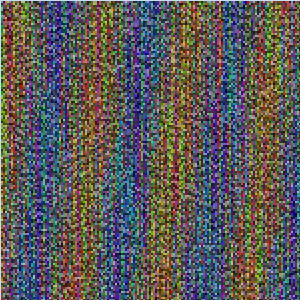
\includegraphics[width=0.9\textwidth]{image/permutation-feif1.png}
    \par Feistel-hálózat (1-round, fast hash)
  \end{minipage}
  \hspace*{\fill}

  \caption[Permutációk kimeneteinek összehasonlítása]{
    A \texttt{Permutation} különféle implementációinak kimenetei
  }
\end{figure}


\section{Egyoszlopos kereshető értékkiosztások}

\subsection{Általános megfontolások}

Olyan értékkiosztási módszereket veszek most végig,
amelyek biztosítják az alábbiakat:

\begin{enumerate}
  \item hatékony pozíció-alapú elérés (random access)
  \item hatékony kereshetőség valamilyen formában
  \item hatékony rendezés
  \item lekérdezések közötti konzisztencia
\end{enumerate}

Az egyes esetekben megvizsgálom majd, hogyan teljesíthetők ezek az elvárások.

\subsection{Keretrendszer az értékkiosztásokhoz}

Alapesetben az adatokat oszlop-orientáltan fogjuk előállítani.
Minden oszlophoz tartozik majd egy virtuális adatlista,
melynek hossza egyenlő az adott oszlopot tartalmazó tábla hosszával.
Opcionálisan szerepelhetnek benne $NULL$ értékek,
a többi érték típusának pedig kompatibilisnak kell lennie az oszlophoz megadott típussal.

Bár ez a megközelítés oszloponként független adatlistákra van szabva,
valójában más jellegű értékkiosztási módszer is lehet mögötte,
amennyiben az egy-egy oszlophoz tartozó listanézetek biztosítottak.
Majd a több oszlopot érintő megkötések esetében ez lesz a helyzet.
De lássuk először az egyoszlopos értékkiosztások lehetséges módszereit.

\subsection{Általános kétlépéses értékkiosztás}

Talán a leggyakoribb eset,
hogy előre ismert véges értékkészlet elemeit szeretnénk viszontlátni az oszlopban,
mégpedig összevissza.
Fentebb már utaltam rá, hogy ez a legtöbb esetben megoldható két független lépéssel.
Először egy \texttt{Monotonic} példány segítségével a kívánt célhosszra
értelmezett függvényt állítunk elő, mely az értékkészlet pozícióira mutat
(ezt a továbbiakban \textit{rányújtás}nak nevezem majd).
Majd az így előállt (esetlegesen $NULL$ értékekkel kiegészített) listát
egy \texttt{Permutation} példány segítségével elkeverjük.

\begin{figure}[H]
\centering
\includesvg[width=0.55\textwidth]{diagram/distribution}
\caption[A kétlépéses értékkiosztás alapelve]{
    A kétlépéses értékkiosztás alapelve:
    egymás után végrehajtott visszafejthető disztribúció és permutáció
}
\end{figure}

Láttuk, hogy mindkét függvénytípus interfésze úgy van definiálva, hogy relációként megfordítható.
A \texttt{Monotonic} \texttt{indicesOf()} metódusaival egy értékindexnek illetve -sávnak
a céllistabeli sávjára tudunk rákérdezni.
A \texttt{Permutation} pedig az \texttt{indexOf()} metódust biztosítja hasonló célra
(illetve inverze maga is permutáció).
Ezek használatával egy reverse index könnyen implementálható.

A még keveretlen rányújtott adathalmazbeli találati sáv határai
egyúttal azonnal megadják a találatok számosságát,
ami egyszerűbb \texttt{COUNT} lekérdezéseknél igen előnyös.

A következő két ábra szemlélteti az adatlekérés illetve értékkeresés folyamatát:

\begin{figure}[H]
  \centering
  \begin{minipage}[t]{0.48\textwidth}
    \includesvg[width=\textwidth]{diagram/getvalue}
    \caption{Adatlekérés a kétlépéses értékkiosztásból}
  \end{minipage}
  \hspace*{\fill}
  \begin{minipage}[t]{0.48\textwidth}
    \includesvg[width=\textwidth]{diagram/findvalue}
    \caption[Keresés a kétlépéses értékkiosztásban]{
      Keresés a kétlépéses értékkiosztásban:
      a rendezett értékkészlet és a leképezések megfordíthatósága
      biztosítja a hatékony keresést a virtuális listában
    }
  \end{minipage}
\end{figure}

\subsubsection{Kétlépéses értékkiosztás gyakoriságtáblázattal}

Egyes esetekben előre ismert az értékek eloszlása,
amit szeretnénk nagyjából vagy pontosan viszontlátni a céloszlopban.
Ekkor egyszerűen a \texttt{Monotonic} fentebb tárgyalt konkrét eloszlásokat használó
implementációnak egyikét kell használnunk.

A felhasználó számára biztosítani kell a gyakoriságok könnyű konfigurálhatóságát,
ehhez érték-gyakoriság párokat kérünk be.
A második érték egymáshoz képesti relatív gyakoriságot jelöl.

\subsubsection{Zajosan monoton értékkiosztások}

A rányújtásnak az előzőleg monoton függvény előállításához használt elve
másféle értékkiosztáshoz is felhasználható,
nevezetesen olyan (szigorúan vagy nem szigorúan) monoton adatsor előállításához,
melynek egyes értékei összességében egy adott sűrűség szerint növekednek
(vagy csökkennek; az egyszerűség kedvéért most csak a növekedő esetről lesz szó),
de lokálisan nagy az egyenetlenség.
Ezt is két lépésben fogjuk megvalósítani.\footnote{
  A két lépés általánosítható egy általános sűrűségfüggvény és egy zajfüggvény összegévé,
  ahol a sűrűségfüggvény meredeksége és a zajfüggvény kilengése közötti megfelelő viszonyt kell biztosítani,
  hogy az értékek ne ugorják át egymást.
  Itt most nem foglalkozom ezzel az általánosabb kerettel.
}

Az első lépés alapelve tehát hasonló az előbbi megoldás első fázisához.
Ám itt nem lehetséges értékeket vetítünk ki a tábla hosszára,
hanem a táblahossznyi alaphalmazt vetítjük majd ki egy diszkrét lehetséges értékkészletre.
Minden sorindexhez hozzárendelődik egy (a szigorú monotonitás elvárása esetén nemüres)
dedikált sáv az értékkészletből.

A második lépés választ egy értéket a sávból.
Nem szigorúan monoton értéksor esetén megengedjük az üres sávot is,
és ilyen esetekben mindig a rákövetkező elemet választjuk.\footnote{
  Ebben az esetben explicite ki kell zárni, hogy az utolsó sáv üres legyen.
  Ez legtermészetesebben egy logikai paraméter beiktatásával érhető el,
  amelyet a rekurzió során mindig csak a felsőbb sávra küldünk tovább \texttt{true} értékkel
  (a többire \texttt{false} értékkel),
  alapértelmezett értéke \texttt{true}.
  Ha tehát \texttt{true} értéket kaptunk, biztosítani kell, hogy az aktuális felsőbb sáv ne legyen üres.
}

Az érték elérése ekkor úgy történik, hogy először lekérjük az értéksávot a rányújtó függvénytől,
majd meghívjuk az értékválasztó függvényt,
melynek paraméterei az értéksáv, a sorindex és a \texttt{TreeRandom}-ból vett seed lesznek.
Egy kézenfekvő megvalósítás,
hogy a seed alapján inicializált véletlengenerátorral
generáltatunk egy véletlen értéket, ami a sávba esik.

Értéksávra való kereséskor vesszük a minimális és a maximális keresett értéket,
és az inverz rányújtást használva megkeressük a megfelelő sorindexeket, amelyek sávjához az érté tartozik.
Ezen sorindexek feszítik majd ki a találati sorindexsávot.
Hogy az alsó érték beletartozik-e, annak eldöntéséhez le kell generálni
az alsó sorindexhez a konkrét értéket, és ellenőrizni, hogy nagyobbegyenlő-e,
mint a keresett alsó érték.
A felső érték esetében hasonlóan kell eljárni.

A rendezés triviális, mivel az értékek eleve rendezettek.

Ezzel az eljárással nem csak zajossá tudtuk tenni az eloszlást,
de a monotonitás garantálása mellett megengedtük,
hogy az értékek esetlegesen csomósodhassanak,
illetve elméletben tetszőlegesen eltávolodhassanak attól a helytől,
amit egy szigorúan egyenletes kiosztás esetén vettek volna föl.

Ez az értékkiosztás különösen alkalmas időbélyegek szimulálására,
amikor az események általános sűrűsége adott,
de véletlenszerű, zajos kimenetet szeretnénk látni.

\subsection{$NULL$ értékek kezelése}

Általánosan, bármely értékkiosztási módszerhez könnyen hozzáilleszthető a $NULL$ értékek támogatása.
Ekkor a rányújtást a tábla méreténél kisebb intervallumra végezzük,
a maradék helyeket pedig egyszerűen $NULL$-nak tekintjük.
A permutáció alkalmazása után a $NULL$ értékek is szétszórtan szerepelnek majd.

Nem szükséges ez a plusz kompozíció,
ha a fentiek magába az eredeti értékkiosztásba is könnyen beépíthetők.
Akár beépítetten, akár plusz kompozícióval van megvalósítva a $NULL$ értékek kezelése,
természetesen figyelni kell a speciális kezelésre a keresés-rendezés során.

A fentiek fényében az egyes értékkiosztások tárgyalásánál a $NULL$ értékek kezelésével nem foglalkozom.

\subsection{Egyszerű értékkiosztások}

Tényleges adatbázisokban némely esetben meglehetősen következetes módon
szerepelnek az értékek az oszlop értéklistájában.
Természetesen az ilyen esetek szimulálása a legegyszerűbb.

Triviális eset, ha egy oszlop mezői egy közös konstans értéket tartalmaznak.

A szekvenciális oszlopoknál az érték megegyezik a rekord 1-től indított sorszámával,
de sok egyéb oszlop is generálható szekvenciális alapon
(feltehetjük, hogy nem történt még releváns módosítás,
ez aztán az írási réteg használatával korrigálható).
Az ilyen esetekben az $n$-edik érték lekérése
egy egyszerű lineáris függvénnyel számolható,
és az érték keresése is hasonlóan történik.

Időbélyegeket is generálhatunk hasonló módon,
amennyiben megengedhető, hogy a szimulált időadatok között egyenletes időközök legyenek.

\subsection{Unique értékkiosztás}

Elsődleges vagy más egyedi kulcsok szimulálásakor fontos,
hogy ugyanaz az érték ne forduljon elő kétszer az értéklistában.
Ennek természetesen előfeltétele,
hogy a lehetséges értékkészlet nagyobb legyen, mint az oszlop hossza
($NULL$ értékek nélkül).

Egyszerűen megvalósítható módszer,
amikor egy permutációt alkalmazunk az értékkészlet fölött,
és a permutált lista oszlophosszúságú prefixét vesszük értéklistaként.
Ekkor a random elérés triviális: csak a permutációt kell visszafejteni.
A keresés a rendezett értékkészletre alapozható,
a találatokat a permutációval megforgatva kell listázni,
kihagyva a prefixen kívül eső értékeket.

Ha azonban az értékkészlet mérete lényegesen nagyobb, mint az oszlophossz,
jellemzően nagyon sok értéket kell átugranunk, amely a prefixen kívül esik.
Ilyenkor sokkal hatékonyabb,
ha az általános kétlépéses értékkiosztást használjuk
egy megfelelő \texttt{Monotonic} implementációval,
akár egyszerű diszkrét lineáris vetítéssel.


\subsection{Reguláris kifejezésből képzett értékkészletek}

\subsubsection{Reguláris kifejezésből generált szó-fák}

Karakterláncokból álló értékkészletnek egy reguláris kifejezés (minta)
alapján történő generálása talán a legáltalánosabb és legrugalmasabb módja
az értékek definiálásának.
Emiatt ezzel a résztémával fogok a legrészletesebben foglalkozni.

Véletlenszerű karakterláncok reguláris kifejezés alapján történő generálására
számos könyvtár elérhető a Java környezethez
(például a \textit{xeger} és a \textit{generex})
\todoref{+CITE: Xeger és Generex}.
Ezek olyan automaták, melyek az állapotgráfot véletlenszerű választásokkal járják be.
Ez a megközelítés önmagában nem alkalmas arra,
hogy az összes illeszkedő karakterláncból álló virtuális értékkészletet
a számunkra megfelelő módon implementálni lehessen vele.
Nem tudjuk ugyanis lekérni a rendezett értékkészlet $n$-edik elemét,
és nem tudjuk kikeresni, hogy adott érték mely pozíción található az értéklistában.

Lássuk, hogyan tudnánk valami módon mégis egy rendezett értékkészletet implementálni.
Egy olyan memóriabarát adatstruktúrát kell előre legenerálni,
melyet futásidőben a gyors lekéréshez és kereséshez használhatunk majd.
Első megközelítésben a reguláris kifejezéssel kapcsolatban az alábbi megszorításokat tesszük:

\begin{itemize}
    \item a minta csak konstans karakterek, karakterosztályok, csoportok és alternációk szerepelnek
    \item a rendezés karakterenkénti, azaz nincs másodlagos, harmadlagos stb. összehasonlítási szempont
\end{itemize}

Ilyen megkötések mellett a reguláris kifejezéshez problémamentesen rendelhető egy
irányított körmentes szógráf (DAWG),
melyben egy érték nélküli kiinduló elemből érjük el a karaktereket reprezentáló csomópontokat,
és kizárólag a szóvég csomópontokon (EOW) terminálhatunk,
melyekből már nem érhető el további csomópont.\cite{AppelScrabble1988}

A gráf lényegileg egy prefix fa, ahol egyes azonos részfákat újrahasznosítunk.
Ezért a továbbiakban az egyszerűség kedvéért néha faként fogok a gráfra hivatkozni.
A gyökértől az adott részfáig vezető útvonalra
néha az adott részfa \textit{prefixeként} fogok hivatkozni.
Az újrahasznosítás miatt a fa tárhelyigénye a reguláris kifejezéshez képest lineáris.
A szóvég csomópontok lesznek a fa levelei.
A prefix fa könnyen felépíthető a reguláris kifejezés szintaxisfájából (AST).
A gráf tömöríthető úgy, hogy konstans karakterek helyett karakterosztályokat engedünk meg.

A felépítés két lépcsőben történik.
Először egy nyers fát állítunk elő, ami közvetlenül reprezentálja a reguláris kifejezést.
\algorithmref{regex_wordtree_create_raw}

Például a \texttt{([a-c]z(tt|uu)r|a[x-z])} reguláris kifejezés nyers szófája így néz ki:

\begin{figure}[H]
\centering
\includesvg[width=0.9\textwidth]{diagram/trie-simple-raw}
\caption{Egyszerű reguláris kifejezés nyers szófája}
\end{figure}

A nyers fa nagyon hasonlít egy szintaxisfához,
a fő különbség, hogy az alternációk vége tovább van csatlakoztatva a külső szekvencia
következő eleméhez tartozó csomóponthoz
(a példában a \texttt{[t]} és az \texttt{[u]} csatlakozik így az \texttt{[r]}-hez).
Ebből világos, hogy a nyers fa mérete és előállításának költsége
a reguláris kifejezés méretével egyenesen arányos.

Látható, hogy a szekvenciákból láncolás lett,
az alternációkból pedig egy több elágazással (gyermekelemmel) rendelkező üres csomópont.
Az is látható, hogy néhány rákövetkező karakter duplikáltan szerepel egyes elágazásokban
(például az '\texttt{a}' betű rögtön az elején).

A közbeékelődő üres csomópontok és a duplikációk miatt
a szófa alkalmatlan arra, hogy keressünk benne,
illetve hogy rendezetten iteráljunk a csomópontokon.
A probléma kiküszöbölésére második lépésben egy normalizálási eljárást hajtunk végre,
mely után a gráfban adott csomópontból elérhető csomópontok listájára az alábbiak érvényesek:

\begin{itemize}
    \item \textbf{explicit terminálás:} a lista opcionális eleme a szóvég csomópont, ami kötelező, ha egyébként nincs más a listában; kivételt képez maga a szóvég csomópont, melynek soha nincs gyermeke
    \item \textbf{egyértelműség:} a lista elemei ezen kívül diszjunkt karakterosztályok
    \item \textbf{rendezettség:} bármely karakterosztály listaelem minden tartalmazott karaktere későbbi, mint bármely megelőző karakterosztály listaelem bármely tartalmazott karaktere; a szóvég csomópont mindig első elem
\end{itemize}

Ezek a szabályok biztosítják, hogy a gráf bejárása rendezett sztringeket ad,
valamint egy trie-szerű adatstruktúrát kényszerítenek ki, amelyben hatékonyan tudunk keresni.

Az átalakítás rekurzív módon történik.
Ahol egymásnak alternatíváját jelentő két karakterosztály között átfedés vagy átugrás van,
ott mindkét karakterosztályt szét kell bontani úgy,
hogy a kapott karakterosztályokból képzett halmazra a fentiek érvényesek legyenek.
Például ha az \texttt{[a-c]}, \texttt{[cf]} és \texttt{[c-e]} jelennek meg alternatívaként,
akkor ezek szétbomlanak az \texttt{[ab]}, \texttt{[c]}, \texttt{[de]} és \texttt{[f]}
karakterosztályokra, és átveszik a korábbiakból elérhető csomópontokat.
A \texttt{[c]} karakterosztály egy alternációt vesz át a három eredeti csomópontból.
A fát egyúttal célszerű úgy továbbalakítani, hogy megszüntetjük az alternációk miatti üres értékű,
pusztán az elágazás kedvéért felvett csomópontokat,
ez természetesen az egyenlő csomópontok részfáinak összefésülését vonja maga után.
Nevezzük az így nyert gráfot a reguláris kifejezés kompakt szófájának.
\algorithmref{regex_wordtree_create_compact}

A \texttt{([a-c]z(tt|uu)r|a[x-z])} reguláris kifejezés fenti nyers szófájából
az alábbi kompakt szófát nyerjük:

\begin{figure}[H]
\centering
\includesvg[width=0.9\textwidth]{diagram/trie-simple-compact}
\caption{Egyszerű reguláris kifejezés kompakt szófája}
\end{figure}

Minden csomóponthoz hozzárendeltük a hozzá tartozó részfa leveleinek effektív számát,
ami rekurzióval könnyen számítható.
Ez az információ már elegendő ahhoz, hogy kikeressük az $n$-edik elemet,
illetve hogy megkeressük egy adott karakterlánc (megtalált vagy beillesztési) pozícióját.

A kompakt szófában megtalálható különböző részfák száma
a nyers szófa különböző részfáinak számához képest exponenciálisan megnőhet.
Induljunk ki ugyanis egy $n$ elemű $C$ karakterhalmazból,
és képezzük rendre a $C_1, C_2, \cdots, C_{n-1}, C_n$ karakterosztályokat úgy,
hogy $C_i$-t $C$-ből az $i$-edik karakter kihagyásával nyerjük.
Képezzük azt az $n$ ágú alternációt,
ahol az $i$-edik ág $C_i$\texttt{\{}$n$\texttt{\}} alakú.
Világos, hogy a reguláris kifejezés által megengedett összes $n-1$ hosszú prefixekben
szereplő karakterek lehetséges halmazai kiadják
$C$ összes legfeljebb $n-1$ elemű halmazait,
ami exponenciálisan növekszik $n$ növelésével.
Minden ilyen halmaz az alternáló ágak egyedi kombinációját azonosítja
(ebben a konkrét esetben ez azt jelenti, hogy különböző lesz a lehetséges utolsó betűk halmaza),
tehát egyúttal legalább ennyi különböző részfa is van.

Az előbbi reguláris kifejezés lényegileg azt fejezi ki,
hogy a karakterláncban nem szerepelhet $C$ összes eleme, ezen kívül bármit megengedünk.
Az ehhez hasonló konfigurációk szerencsére meglehetősen életszerűtlennek tűnnek.
Az ilyen szempontból problémás alternációkat akár előre is detektálhatjuk,
és túl nagy becsült növekedés esetén expliciten hibát dobhatunk.

Most pedig nézzük hogyan tudunk engedni a fenti megszorításokon.

A repetíciós operátorok explicite kifejtés által kerülnek visszavezetésre a fentiekre.
A kifejtés természetesen egyes esetekben lényegesen megnövelheti a fa méretét a bemenethez képest.
Ennek kioptimalizálásával most nem foglalkozom.

Először a korlátlan repetíciót (\texttt{*}, \texttt{+} stb.) elimináljuk rendre az alábbi szabályokkal:

\begin{enumerate}
    \item \texttt{$A$+} ~ $\longrightarrow$ ~ \texttt{$A$\{1,\}}
    \item \texttt{$A$\{$n$,\}} ~ $\longrightarrow$ ~ \textt{$A$\{$n$\}$A$*}
    \item \texttt{$A$*} ~ $\longrightarrow$ ~ \texttt{$A$\{$c$\}} ~~~~~ (ahol $c$ előre definiált konstans)
\end{enumerate}

A fix repetíció egyszerű konkatenációvá alakul,
az opcionális repetíció kifejtése pedig a következő rekurzív módon történik:

\begin{enumerate}
    \item $R_1~=$ \texttt{$A$\{,1\}} ~ $\longrightarrow$ ~ \texttt{($A$|)}
    \item $R_n~=$ \texttt{$A$\{,$n$\}} ~ $\longrightarrow$ ~ \texttt{($AR_{n-1}$|)} ~~~~~ (ahol $n>1$)
\end{enumerate}

Az opcionális előfordulás (\texttt{?}) az $R_1$ esettel egyenlő.

A támogatott konstrukciókat könnyen tovább bővíthetjük az egyszerűbb horgonyokkal,
mint például szövegvég (\texttt{\$}) vagy szóhatár (\texttt{{\textbackslash}b}).
Ezeket a kezdeti feldolgozáskor úgy tekintjük,
mint az átmeneti üres csomópontokat, tehát elimináljuk és megjegyezzük őket,
de utána sorban kikényszerítjük a teljesülésüket.
A horgonynak ellentmondó gyermekelemeket eltávolítjuk,
ha ezután nem marad gyermekelem, a teljesíthetetlen ágat jelző kivételt dobunk,
a kivételt elkapó szint el fogja dobni az ágat mint lehetetlent,
ami újabb kivételdobást eredményezhet, ha az ottani gyermekelemek emiatt elfogytak,
és így tovább.

\subsubsection{Unicode karakterláncok és többszintű rendezés reguláris kifejezésekkel}

Az igazi nehézségek akkor kezdődnek,
amikor elengedjük a karakterenkénti rendezés megszorítását
(ami természetesen további többletköltségeket fog eredményezni,
ezért érdemes opcionálissá, konfigurálhatóvá tenni).
Erre például ékezetes karakterek vagy kis- és nagybetűk keveredése esetén lehet szükségünk.
Ekkor ugyanis esetleg csak egy későbbi eltérés dönti el,
hogy egy korábbi ékezet vagy nagybetűsség számít-e.
Vagyis az egyszerű, karakterenkénti prefix-fa sem elég a rendezettség biztosításához.

Ha egy ilyen szofisztikáltabb rendezési elvet akarunk megvalósítani,
az \textit{Unicode Collation Algorithm} (UCA) szabványból érdemes kiindulni\protect\cite{UCA2024}.
A UCA azonban rendkívül összetett,
így egyelőre csak az alapvető szempontok implementálását fogom bemutatni.
Ki-kitérek majd arra, hogyan lehet ezeket a későbbiekben bővíteni, továbbfejleszteni,
hogy még részletesebben lefedje a szabvány által tárgyalt lehetőségeket.

A UCA mindenekelőtt definiál egy általános keretrendszert,
mely egy sémát ad arra, hogyan kell többszintű rendezéseket megvalósítani Unicode karakterláncokon.
A sémát implementáló konkrét algoritmusokat \textit{kollációknak} nevezzük.
Egy Unicode karakterlánc lényegileg Unicode codepoint-ok tömbjét jelenti
(Java környezetben a \texttt{char} adattípus ilyen codepointot tárol).
Egy kolláció egy-egy ilyen tömbhöz rendezési szintenként hozzárendel egy-egy
kollációselem-listát (\textit{Collation Element Array}).
A kollációs elemek lényegileg codepointok, de a kolláció által definiált súlyozás szerint átszámozva.
Tehát úgy is felfoghatjuk, hogy a kolláció a Unicode karakterlánchoz
szintenként egy másik Unicode karakterlánc nézetet rendel,
ahol a codepointok között egyúttal egyedi sorrendezést definiál.
A UCA öt alapértelmezett rendezési szintet különböztet meg:

\begin{itemize}
    \item \textbf{L1}: alapkarakterek (Base characters)
    \item \textbf{L2}: diakritikus jelek (Accents)
    \item \textbf{L3}: kis-/nagybetűsség (Case/Variants)
    \item \textbf{L4}: írásjelek (Punctuation)
    \item \textbf{Ln}: kódolási különbségek (Identical)
\end{itemize}

Például a normál magyar kollációban a '\texttt{Kör}' karakterlánc L1-es alakja '\texttt{kor}'
ahol a diakritikus jel és nagybetűsség stb. ignorálásra (eltávolításra) került.
Ellenben például a svéd nyelvben az '\texttt{ö}' betű az ABC végén
teljesen különálló betűként szerepel,
így a normál svéd kollációban a fenti karakterlánc L1-es alakja '\texttt{kör}',
és a rendezésben is egészen máshogy fog viselkedni.

A UCA szerint két karakterlánc összehasonlításakor sorban vizsgálandók az egyes szintek,
míg az egyik szerint különbséget nem találunk.
Ekkor egyszerűen a kollációselem-listák elemenkénti összehasonlítása szerint
kerül megállapításra a két karakterlánc egymáshoz képesti sorrendje.

Az \textit{International Components for Unicode} a Unicode Consortium hivatalos
referenciaimplementációja általában a Unicode szabványhoz,
beleértve számos konkrét kollációt a világ nyelveihez~\protect\cite{ICU2024}.
Konkrét szabályok kialakításához ebből érdemes kiindulni.
Az ICU általában (beleértve a standard, európai és magyar kollációkat is)
teljesen az L1 szinten kezeli az írásjeleket is
(az egymás utáni több írásjel is külön-külön elsődleges karakternek számít).
Ez logikusabb, mint az írásjeleket egyáltalán nem figyelembe venni a betűk vizsgálatakor,
hiszen akkor a szavak tagolása sem történik meg
(például az '\texttt{ab:cd}' előrébb kerül, mint az '\texttt{a:cd}').
Ezt is figyelembe véve, mi most csak az első három szinttel foglalkozunk,
legalábbis kizárólag pozíciótartó összehasonlításokkal.

A kompakt szófa fentebbi implementációját a következő ötlettel tudjuk kibővíteni
a többszintű rendezés támogatásához.
Minden rendezési szinthez külön szófát készítünk, melyeket az eredeti szófa egyszerűsítésével nyerünk
(az életszerűség csorbítása nélkül feltehetjük,
hogy a reguláris kifejezés olyan, hogy ez problémamentesen megtehető).
Ekkor az egyszerűsített fákban egy-egy maximális útvonalhoz 1-nél több eredeti karakterlánc tartozhat
(az egyszerűsítés éppen ezt az összevonást jelenti
az adott szinten egyenlőnek számító karakterláncok között).
Ezeket a szófákat aztán (virtuális értelemben) egymás alá fűzzük,
azaz effektíve minden előző szint EOW csomópontja után konkatenáljuk a következő szint fáját.
Az összevont (például egybeolvadó karakterekhez tartozó) részfák
többszörös számossággal számítanak, amit jelezni kell.

Az n-edik karakterlánc lekérése úgy történik,
hogy az egymás alá fűzött fák rendszerében (ami maga is egy nagy faként értelmezhető) navigálunk.
Az első fában normál módon keresünk, azzal a kiegészítéssel,
hogy a szorzó csomópontok egyszerűen olyan részfák listájaként értelmezendők,
melyek a szorzó csomópont gyermekelemeihez tartozó részfákkal egyenlők,
azonban minden méretükben a szorzóval növelve.
A levélhez érve a szorzók miatt egy 1-nél nagyobb számosságot kaphatunk.
Ezt a számosságot a további szintek részfái fogják tovább-bontani.
Az utolsó szint kivételével mindegyik fában megengedett (sőt, a dolog lényegéhez tartozik)
a többszörös számosság.

Világos, hogy (a szorzókat figyelembe véve) egy-egy szint fája
a teljes eredeti értékkészlet számosságával bír.
Amikor azonban már a többedik fában kezdünk továbbmenni,
valójában a fa olyan szűkített nézetét kell vennünk,
amely kompatibilis az összes már előbbi szint fájában bejárt útvonallal.
Például (magyarral kompatibilis kollációs szabályokat feltéve),
ha az első szinten a '\texttt{tarol}' karakterláncot kaptuk,
a második szint fája megengedheti a '\texttt{tarol}', `\texttt{tárol}', '\texttt{táról}' stb.
karakterláncokhoz tartozó útvonalakat,
de mondjuk a (tegyük föl, eredetileg megengedett) "hasonlít" útvonalát már nem.

Ez a szűkítés a bemenettől függ.
Vagyis nem tudjuk előre generálni, a futási idejű performanciát fogja befolyásolni.
A előbb bemutatott adatszerkezet alkalmas arra, hogy ezt hatékonnyá tegye,
de ehhez szükség van egy lényeges megkötésre,
nevezetesen, hogy az egyszerűsítés pozíciótartó legyen,
azaz egy adott karakterlánc összes szintbeli nézetének hossza egyezzen az eredeti hosszal,
és bármely karaktere a vele azonos pozíción található eredeti karakter derivátuma legyen.
Mivel csak pozciótartó összehasonlításokra szorítkoztunk,
ez a megkötés eleve biztosított.

Karakterlánc keresésekor is a fenti szempontokkal egészítjük ki
a többszintű rendezést nem támogató kompakt fánál látott algoritmus-sémát.
A fő eltérés, hogy a kereséskor nem az addigi útvonalakkal,
hanem a keresett eredeti karakterlánccal való kompatibilitás számít,
nyilván már az első szinttől kezdve.

\subsection{Full-text indexelt értékkiosztás}

Ez az értékkiosztási mód folyószövegeket állít elő, melyekhez full-text indexet tesz elérhetővé.
Itt most csak a full-text index legegyszerűbb fajtájával foglalkozunk,
melynek bemenete egy néhány szóból álló halmaz,
eredménye pedig az ezen szavak mindegyikét tartalmazó mezők sorindexeinek halmaza.
Rendezéssel ez esetben nem foglalkozunk, a full-text indexek ezt általában nem is biztosítják.
Látni fogjuk, hogy a bemutatott megoldás könnyen továbbfejleszthető.

Első körben induljunk ki abból, hogy adott egy szólista, a mellékelt $f_i$ előfordulási gyakoriságokkal.
Az $f_i$ előfordulási gyakoriság szimulálható is a Zipf-törvényre alapozva.
A Zipf-törvény egy számos különböző területen fennálló statisztikai jelenség,
miszerint a diszkrét gyakoriságok általában hatványtörvény szerint rendeződnek (Zipf-eloszlás).
Vagyis egy (némileg paraméterezhető) törvényszerűséget ad meg arra vonatkozóan,
hogy a leggyakoribb, második leggyakoribb stb. elem
milyen gyakorisággal fordul elő a teljes mintában.
A törvényszerűség meglehetősen egyetemesen fennáll az organikusan alakuló rendszerekben,
ezt követi például a jövedelmek, városok, állatok stb. méret szerinti gyakorisága.
Esetünkben azért érdekes, mert a legtöbb természetes nyelvben a szavak gyakorisága is így oszlik el.
\cite{Zipf1942UnityOfNature}.

A szavakat egyszerűen betűkarakterek sorozataiként fogjuk föl,
előzetesen függetlenítve a központozás, szövegfelépítés problematikájától.

Lesz emellett egy a szövegekre vonatkozó várható szószám is, jelöljük ezt $c$-vel.
A gyakoriság és a hossz együtt meghatározza az adott szó
$p_i$ szereplési valószínűségét valamely szövegben a következő egyszerű képlet szerint:

$$
p_i = 1 - (1 - f_i)^c
$$

Legyen $s$ az egy szövegben várhatóan előforduló szavak halmazának számossága ($s \leq c$).
Az $n$ táblahossz számú mezőre akarjuk képezni a szövegeket,
amit egy $n \times s$ méretű virtuális mátrix segítségével fogunk elvégezni.
A szavakat valamilyen sorrendben véve (a sorrend megválasztásának problémáit most mellőzöm),
az $n s$ hosszú listát feltöltjük úgy, hogy minden szó egy összefüggő sávban szerepel,
a sávok sorrendje az említett szósorrend,
a sávok egymáshoz képesti relatív hossza pedig a $p_i$ szereplési valószínűségen alapul.
Ezt a listát képezzük bele oszlopfolytonosan a mátrixba.

Egy adott sorindexhez tartozó mezőben szereplő szavakat úgy kapjuk,
hogy egyszerűen vesszük a mátrix megfelelő sorát.
Szavakra keresni pedig úgy tudunk, hogy a keresett szavakhoz tartozó
(esetleg oszlopváltással megszakított) sávok metszetsávját vesszük,
ha nincs metszet, nincs találat.
A mátrixsorokat az életszerűség kedvéért érdemes permutálni a fentebb már ismertetett módszerrel.

A mátrixos módszer egyik hátránya,
hogy az egymás mellé került szavak eltartanak egymástól ugyanabban az oszlopban,
így jellemzően nem tudnak majd bekerülni ugyanabba a szövegbe,
illetve általában is viszonylag korlátolt,
hogy melyek a lehetséges konstellációk.
Ez viszonylag jól orvosolható azzal, ha egy-egy szó sávja több független sávba törik szét
(jól ügyelve arra, hogy ezek a részsávok távoli sorokra essenek,
de legalábbis ne legyen metszetük modulo $n$).

Egy másik probléma (hacsaknem épp ez a cél), hogy a szövegek túl uniformak, ugyanannyiféle szóból állnak.
Ezen könnyen segíthetünk, ha a szósávok közé sok apró üres sávot helyezünk el.

A következő ábrák szemléltetik az eddig leírt szóösszeállítási illetve keresési módszert:

\begin{figure}[H]
  \centering
  \hspace*{\fill}
  \begin{minipage}[t]{0.42\textwidth}
    \includesvg[width=\textwidth]{diagram/fulltext-getvalue}
    \caption{Full-text szóösszeállítás}
  \end{minipage}
  \hspace*{\fill}
  \begin{minipage}[t]{0.42\textwidth}
    \includesvg[width=\textwidth]{diagram/fulltext-findvalue}
    \caption{Full-text keresés}
  \end{minipage}
  \hspace*{\fill}
\end{figure}
í
Egy harmadik egyszerű javítás adódik,
ha előre ismert, mely néhány (ideálisan kb. 6-8) szó lesz gyakran keresve,
ezeket teljesen külön kezelhetjük.
Vesszük az összes lehetséges előfordulási kombinációt azok pontos gyakoriságával,
az így kapott értékkészletet pedig lineárisan rányújtjuk a táblahosszra.
Célszerű ezt a többi szótól teljesen függetlenül permutálni.
Egy mező szóhalmazaként a kétféle kiosztás unióját kell venni,
kereséskor pedig a kettő által adott találatok metszetét.

Megjegyzem, ha vannak kiemelt szavak, akkor a többi szó halmaza részben vagy egészben
akár mesterségesen előállított szavakból is állhat.
Ekkor egy minta alapján generálunk szavakat
(on-the-fly, ld. a reguláris kifejezések kapcsán írottakat),
majd például a Zipf-törvény alapján hozzájuk rendeljük a gyakoriságokat.
Ha így járunk el, megspóroljuk a konkrét szavak tárolásának tárhelyigényét.

Egy-egy mezőértékhez még csak a szavak halmazát állítottuk elő.
Amikor lekérjük a mező konkrét értékét, akkor egy tényleges szöveget szeretnénk kapni,
mely pontosan ennek a halmaznak a szavait tartalmazza (sorrendtől és multiplicitástól függetlenül),
és lehetőleg egy viszonylag valóságosnak tűnő szöveg, még ha nem is értelmes.
Vegyük észre, hogy ebben teljes szabadságunk van, hiszen az érték és index konzisztenciája már biztosított.

Az aktuális \texttt{TreeRandom}, a sorindex és a kapott szóhalmaz függvényében
a szöveg generálására tetszőleges módszert használhatunk,
itt tehát egy széles skálázási lehetőség adódik.
A fapados megoldás a halmaz szavainak egyszerű felsorolása szóközzel választva
(abban a sorrendben, ahogy a kiemelt szavak fel voltak sorolva, illetve ahogyan a mátrixból nyertük őket).
Egy nagyon szofisztikált módszer lehet, ha nyelvi modellt használunk a szöveg generálására.

Egy olcsó, ugyanakkor viszonylag jó eredményt adó módszer a következő:

\begin{enumerate}
    \item Határozzuk meg a $c_i$ konkrét szószámot.
    \item Vegyük a szóhalmazt valamilyen konkrét sorrendben.
    \item Helyezzünk ezek közé további szavakat, míg a $c_i$ szószámot el nem érjük.
    \item Határozzuk meg a mondat- illetve részmondathatárok pozícióit.
    \item Fűzzük össze a szöveget szóközökkel, adjuk hozzá a központozást.
\end{enumerate}

Mindegyik lépés finomítható különféle heurisztikákkal,
ezekkel most nem foglalkozom.

A fent tárgyalt full-text index természetes módon bővíthető.
Könnyen integrálható például a kizárandó szavak kezelése.
A szóhalmaz kiválasztásának és a szöveg generálásának összehangolásával
a kifejezésekre való keresés bizonyos formái is megvalósíthatóvá válnak.
Ezekre a bővítési lehetőségekre ezen keretek között szintén nem tudunk részletesen kitérni.



\subsection{Földrajzi koordináták értékkiosztása}

A legegyszerűbben közelítjük meg a problémát,
ami nagyobb dimenziószámra és lényegileg tetszőleges geometriára is átvihető.
Csak a megoldás vázát ismertetem.

Az értékek sűrűségének, elhelyezkedésének valamint opcionálisan a várható lekérdezések
figyelembevételével a felületet térszeletekre osztjuk.
Ennek a felosztásnak nem feltétlenül kell egyenletesnek vagy egyáltalán szabályosnak lennie,
de az egyszerűség kedvéért most maradjunk a szokványos hálónál:
adott $w$ földrajzi hosszúságonként illetve adott $h$ földrajzi szélességenként vágjuk föl a gömbfelszínt.
A kapott háló (a sarkoknál háromszöggé fajuló) kis kvázi-négyszögeket határoz meg.
Ezeket soronként véve egy lineáris sorrendezést kapunk.

A szélesség-hosszúság párokat egy $2d$ bites ábrázolással kódoljuk.
Ennek lehetséges értékkészletére nyújtjuk rá a sorindexeket
a zajosan monoton értékkiosztásoknál ismertetett módszer valamely variánsával,
de itt a nagyléptékű egyenletességet más szempontokra cserélhetjük.
Az értékkészlet összefüggő sávjai a kvázi-négyszögeknek feleltethetők meg,
tehát a kvázi-négyszögekbe tartozó értékekre ugyanúgy tudunk keresni,
mint fentebb az időbélyegekre.

Kereséskor a kvázi-négyszögek két halmazát kell elkülöníteni:
amelyek teljesen az alakzaton belülre esnek,
illetve amelyeket az alakzat határvonala átmetsz.
Az előbbiek értékei feltétel nélkül találatok lesznek.
Utóbbiaknál a kvázi-négyszögön belülre kell hatolnunk,
esetleg egyesével kell ellenőriznünk az értékek alakzaton belüliségét.
Mivel ezek a határvonalhoz köthetők,
számuk egyszerű alakzatok esetén a kerülettel egyenesen arányos,
nem kell tehát területarányos mennyiségű kvázi-négyszöget megbontani,
sőt, az egy sorban egymás után lévők összevontan is kezelhetők.

\begin{figure}[H]
\centering
\includesvg[height=0.4\textwidth]{diagram/geospatial-search}
\caption[Geolokációk keresése alakzat alapján]{
    Geolokációk keresése alakzat alapján, rácsozott gömbfelületen. \\
    Csak a határvonal által metszett mezőkbe eső pontokkal kell részletesebben foglalkozni.
}
\end{figure}


\section{Egyéb értékkiosztási módok}

\subsection{Nem-indexelt egyoszlopos értékkiosztások}

A nem-indexelt oszlopok szimulálásakor a keresési-rendezési szempontokat egyáltalán nem kell figyelembe venni.
Az indexelt oszlopokra vonatkozó elvárások közül így csak az első kettő releváns:

\begin{enumerate}
    \item hatékony elérés (random access)
    \item pozíciótól függő érték (\texttt{TreeRandom} seed)
\end{enumerate}

Vagyis elég, ha a \texttt{TreeRandom} által a sorindexhez generált seed alapján
előállítunk egy normál \texttt{Random} példányt,
és ennek felhasználásával a tartalmat tetszőleges determinisztikus módszerrel állíthatjuk elő.
Erre az előállításra kizárólag a konfigurációban megadott beállítások jelentenek megszorítást.

A következő listában csak fölvillantanám az ilyen adattartalmak néhány jellegzetes,
egyúttal könnyen szimulálható típusát:

\begin{itemize}
  \item \textbf{Egyszerű szöveg:}
    a legegyszerűbb megoldásban egy szótár szavait véletlenszerűen helyezzük egymás után,
    közben feljavítva a szövegképet nagybetűs szavakkal és központozással
    (az eredmény tovább javítható kifejezésminták használatával,
    amikor időnként egy többszavas részletre előre adott sablont használunk;
    de ha a minőség az elsődleges, bevethetünk akár
    Markov-láncokra épülő egyszerűbb nyelvi modelleket\cite{Amrrs2021MarkovHeadlines})
  \item \textbf{Strukturált szöveg:}
    először előállítunk egy általános struktúrát (címek, bekezdések stb.),
    majd ennek elemeit feltöltjük szöveggel (lásd az előző pontot),
    végül a struktúrát a kívánt jelölőnyelven szolgáltatjuk (HTML, MarkDown, plain text stb.)
  \item \textbf{Strukturált adat:}
    generált vagy konfigurációban megadott adatséma alapján rekurzívan generáljuk le az adatstruktúrát,
    ekkor a sémanyelv (pl. JSON Schema) és a kimenet formátuma (JSON, YAML, TOML stb.)
    függetlenül konfigurálható
  \item \textbf{Egyszerűbb képek:}
    véletlen színű háttérre véletlen paraméterekkel
    rárajzolunk néhány egyszerű alakzatot,
    majd a kívánt vektoros vagy raszteres formátumban szolgáltatjuk
  \item \textbf{Jelszó-hash:}
    a tényleges a hash-algoritmust hívjuk meg valamely rendelkezésre álló adatra,
    pusztán formai elvárás esetén akár magára a \texttt{TreeRandom} seedre,
    demózáshoz pedig hasznos lehet a felhasználónevet használni jelszóként
  \item \textbf{Általános BLOB/CLOB:}
    lekéréskor a konfigurációban megadott mérethatárok közötti bájtsort/karaktersort kell visszaadni,
    ami könnyen ellátható random bájtok/karakterek generálásával
    (legegyszerűbb közvetlenül a \texttt{TreeRandom} által szolgáltatott biteket használni)
\end{itemize}

További indexeletlen eset, amikor az oszlop teljes tartalma explicite felsorolva van megadva,
például egy listafájlból.
Nagy táblahossznál érdemes lehet ezt indexeltté tenni egy tényleges adatstruktúrával (például B-Tree),
mivel ilyenkor valószínűleg úgysem a memóriahasználat minimalizálása a cél.

\subsection{Értékkiosztás oszlopok közötti összefüggéssel}

Az oszlopok közötti összefüggésnek számtalan módja lehetséges.
A legáltalánosabb eset képletszerű összefüggések felsorolása lenne,
ami indexeletlen esetben meg is megvalósítható:
a \texttt{TreeRandom}-ból nyert seeddel véletlenszerűsítve futtathatunk valamilyen constraint solvert,
mely a követelményeket teljesítő értékeket determinisztikusan előállítja.
Ha lehetséges, hogy egyes seed értékek mellett a követelményrendszer nem kielégíthető,
akkor meg kell engednünk a $NULL$ értékeket az érintett oszlopokban,
és a kielégíthetetlen esetekben mindegyikre $NULL$-t kell visszaadni
(esetleg valamilyen egyéb alapértelmezett értéket).

Szintén elég általános eset, amikor mesteroszlopok
alapján akarunk indexeletlen oszlopokat egymástól függetlenül legenerálni.
Ekkor teljes szabadságunk van,
értelemszerűen a mesteroszlopok értékei és a \texttt{TreeRandom}-ból nyert seed lesz a bemenet.

Életszerű azonban, hogy indexelt mesteroszlopokon túl
a függő oszlopokra is szeretnénk indexelést.
Ha egy nagy közös index elég,
akkor elégséges a függő értékeket becsoportosítani a mesterértékek alá.

Bonyolult, de még mindig teljesen életszerű eset,
amikor a függő értékek külön önálló indexeket is kapnak
(ilyen eset például, ha az életkor adatot a végzettséghez igazítva generáljuk).
Ha a mesteroszlop(ok) értékkészlete kicsi,
akkor minden ilyen értéken belül elvégezhetjük a keresést illetve rendezést a függő értékekre,
és ezek összefésült eredményét adjuk vissza.

\subsection{Táblák közötti kapcsolatok}

Amíg megmaradunk a read-only szempontoknál,
a táblák közötti idegenkulcs jellegű kapcsolatokra vonatkozó egyetlen kemény követelmény,
hogy a hivatkozó tábla érintett oszlopa (vagy oszlop-$n$-ese)
csak a hivatkozott tábla érintett oszlopához (vagy oszlop-$n$-eséhez)
tartozó értékkészlet elemeit vehesse föl;
vagyis ($NULL$ értékektől eltekintve),
a hivatkozó oszlop értékkiosztásakor az alaplista a hivatkozott oszlop tartalma lesz.
Másként fogalmazva, az értéklistát indextartó módon kell átképezni a másik táblára.
Ez a fentiek tükrében már egyszerűen biztosítható.

Egyes esetekben (bizonyos típusú 1:1 kapcsolatok) valójában egy tábla kerül szétbontásra több táblára.
Ekkor a több táblára bontottság csak külsődleges,
és az előző részben oszlopok közötti összefüggésekről írottak alkalmazhatók,
még akkor is, ha a két tábla számossága nem egyezik teljesen
(a hiányzó sorok a $NULL$ értékek kezelésének fentebb ismertetett
általános módszerével kerülhetnek kiválasztásra).

A legbonyolultabb esetben 1:n kapcsolat mellett különféle statisztikai
vagy egyéb követelményeket biztosító indexelt oszlopokat szeretnénk előállítani.
Ennek tárgyalása messzire vezet,
de egy rövid megjegyzéssel érzékeltetném, hogy a dolog nem lehetetlen:
egy lehetséges kiinduló megközelítés, hogy a két táblát egyként kezeljük,
az egyesített táblában a kisebb tábla adatait pedig redundánsan szerepeltetjük
(ez egy oszlopközi összefüggés a fenti értelemben);
így az összefüggéseket már táblán belül tudjuk értelmezni.



\chapter{Gyakorlati eredmények}

\section{Néhány bővítési példaszcenárió}

Eddig általános igényekkel foglalkoztunk,
melyeket a megoldásnak out-of-the-box kell támogatnia.
Alább bemutatok három speciálisabb szcenáriót,
demonstrálva az architektúra bővíthetőségét és rugalmasságát.

\subsection{Valós címadatok használata}

Előfordulhat, hogy bizonyos adatok óriás értékkészletét külső adattárakból szeretnénk betölteni,
amivel ugyan elvesztjük a teljes virtualitás kis memóriaigényét és további kedvező jellemzőit,
de még mindig igényt támaszthatunk az egyéb előnyökre.
Most egy ilyen szcenáriót vizsgálok meg:
valamely tábla rekordjaiban olyan magyarországi közigazgatási címeket szeretnénk viszontlátni,
melyek valósak.
Amennyire lehetséges, indexeket is szeretnénk biztosítani.

A cím elemei különálló mezőkre bonthatók.
Első körben kiválasztjuk azokat, melyek egy egyértelmű hierarchiát definiálnak:

\begin{center}
    településnév ~ $\rightarrow$ ~
    kerület ~ $\rightarrow$ ~
    közterület neve ~ $\rightarrow$ ~
    közterület jellege ~ $\rightarrow$ ~
    házszám ~ $\rightarrow$ ~
    egyéb
\end{center}

Az „egyéb” részt nem szofisztikáljuk tovább, egy szabad szöveges mezőnek tekintjük.

Néhány további mező nem tartozik a fő hierarchiába:

\begin{center}
    település típusa ~ $\bullet$ ~
    vármegye ~ $\bullet$ ~
    irányítószám
\end{center}

Utóbbi mezőkre külön-külön indexeket fogunk biztosítani.
A fő hierarchiára pedig egy közös többoszlopos (leftmost prefix) indexet,
pontosabban kettőt:
lesz egy rövidített változat vidéki címekhez, melyben a kerületet nem kell megadni,
és implicite üres értékkel töltődik, amikor továbbhív a másik indexre.

A címadatbázist egy nagy fastruktúrába rendezzük,
minden szintnek a fenti hierarchia egy-egy eleme felel meg.
Az alsóbb szinteken spórolhatunk a tárolással,
például egymásutáni megbontatlan házszámok tartományként tárolhatók.
Egy prefix indexhívásnál a megfelelő szintig megyünk le a keresésben,
a találatok pedig az az alatti levelek lesznek.
A tényleges rekordokra való leképezést
a kétlépéses értékkiosztásnál megismerthez hasonló módszerrel végezzük el.

A fő hierarchián kívüli mezők értékei és a fa közötti indexelést külön adatstruktúrába generáljuk.
Változó lehet, hogy a tábla mely szintjén történik meg az irányítószámra való leképezés,
a legtöbb helyen egy egész várost tudunk hozzárendelni.

\subsection{Valószerű geográfiai értékek előállítása}

A probléma: földrajzi koordinátákhoz akarunk valamilyen számszerű adatot kapcsolni úgy,
hogy mindkettőhöz külön index tartozik,
és a koordinátával ellátott adatok valamilyen szempontból valószerű elrendeződést mutatnak.
Olyan megoldást kell találni, ahol tetszőleges számú ilyen kapcsolt adat akár függetlenül generálható
(különben elég lenne a szélesség-hosszúság-adat háromdimenziós terében megfelelően alkalmazni
a földrajzi koordináták fentebb ismertetett értékkiosztását).

Az alapötlet rendkívül egyszerű, és kellően rugalmas.
Szükségünk lesz egy $F$ függvényre, mely minden földrajzi koordinátához rendel egy kapcsolt értéket.
A kapcsolt adat értékkészletét kis sávokra bontjuk föl (nevezzük ezeket kontextussávoknak),
és minden sávhoz le kell tudnunk kérni azon alakzatok (véges) listáját,
melyekben az $F$ függvény értéke a sávba esik.
Bármilyen függvény megfelel, ha ezeket tudjuk biztosítani hozzá.
Használhatunk például teljesen virtuális háromszögelt felületet,
ahol egy-egy háromszög mindig egy konkrét értéksávba esik, nem nyúlik át.
Vagy akár betölthetünk tényleges domborzati adatokat.

Ha ezt sikerült megoldani, az értékkiosztás működése már triviális.
Adott rekordhoz a földrajzi koordinátát a korábban ismertetett módszerrel generáljuk,
a kapcsolt adatot ez alapján számítjuk az $F$ függvény szerint.
A kapcsolt adat valamely egyéni értéksávjára való kereséskor
lekérjük a sávon teljesen belülre eső illetve a kilógó kontextussávokat,
lekérjük az ezekhez tartozó alakzatokat,
és ezen alakzatokra keressük a földrajzi koordinátákat.
A keresett sávon teljesen belülre eső kontextussávokhoz tartozó találatok feltétel nélkül megtarthatók.
A kilógó kontextussávokban le kell kérni a konkrét kapcsolt értéket,
és eldobni a találatot, ha az mégsem esik a keresett sávba.

\subsection{On-demand schema}

Egyes használati esetek megengedik,
hogy további drasztikus lépésként teljesen nyitottá és automatikussá tegyük a virtuális adatbázis felépítését.
Ebben az esetben konfigurációs fájl létrehozására sincsen szükség,
mindent a beérkező kérések alapján fogunk generálni.
Itt feltételezem, hogy csak olvasási műveletek érkeznek,
de az elv, komoly komplikációk vállalásával, írható műveletekre is kiterjeszthető.

Néhány alapbeállítást (pl. \texttt{seed}) beégethetünk, vagy az első lekérés függvényévé tehetünk.

A táblás lekérések implicite megadnak valamilyen szerkezetet,
mivel konkrét sémákon és táblákon belüli konkrét oszlopokat próbálnak elérni.
Ezeket on-demand kell létrehozni, és a továbbiakban megtartani.
A táblák hosszának beállításakor esetleg figyelembe vehetjük az első lekérés limit értékeit, ha van.
Az oszlop paramétereit a lekérésben az adott oszlopra vonatkozó
implicit információk alapján kell meghatároznunk.
Az oszlopnév, az érték használati módja, a keresési feltételek stb.
mind hasznosak lehetnek.
Ha nem tudtuk eléggé leszűkíteni az oszlop típusát,
valamilyen kellően generikus alapértelmezett beállítást kell használnunk,
ekkor is vállalva persze, hogy egy jövőbeli lekérdezés ezzel inkompatibilis lesz.

A wildcardos lekérdezéseknél többféle stratégiát követhetünk,
legegyszerűbb, ha egyszerűen az addigi oszlopokat adjuk vissza
(új tábla esetén egy alapértelmezett oszlopot adhatunk hozzá).

A szisztéma megvalósításához mindössze egy proxy réteg szükséges,
mely minden beérkező kérés továbbítása előtt megfelelően kiegészíti a konfigurációt,
és újratölti a virtuális adatbázist, ha szükséges.
A \texttt{TreeRandom} hierarchia természetéből adódóan a korábbi oszlopok
továbbra is ugyanazokat a konkrét értékeket fogják szolgáltatni.


\section{Empirikus eredmények}

\subsection{Mérési módszertan}

Mivel a HoloDB preparálási folyamat nélkül rendelkezésre áll,
lényegileg azonnal elindul és minimális memóriát fogyaszt,
ezekben a paraméterekben nem volt értelme összevetni
a radikálisan eltérő opciókkal.
Így alapvetően a lekérdezési sebességre koncentráltam,
azt szűk keresztmetszetében és end-to-end jellegű integrált tesztekkel is megvizsgáltam.
A performanciával kapcsolatban a várakozás mindössze annyi volt,
hogy legyen összemérhető a valódi adatbázisokéval.
A Docker-képek összehasonlítását leszámítva minden esetben
a HoloDB beágyazott verzióját használtam.
Az összehasonlítást MySQL-lel (mint az egyik legelterjedtebb szerveradatbázissal)
és H2-vel (mint a Java környezetben legelterjedtebb beágyazott adatbázissal) valósítottam meg.
A lekérdezések közvetlen mérésénél az SQL parancsnak a JDBC API-n keresztüli beküldésétől
az eredménytábla végigiterálásnak végéig eltelt időt mértem.
Különböző bonyolultságú és válaszméretű lekéréseket vizsgáltam.

Az integrált tesztelést egy Micronaut keretrendszerben implementált
alkalmazás REST API-n keresztüli hívásával futtattam.
A Micronaut keretrendszer egy kis erőforrásigényű Java keretrendszer,
amely minimális erőforrás-lábnyománál fogva a legalkalmasabbnak tűnt a mérésre.

A Spring és Quarkus rendszerekkel szemben a Micronaut már fordítási időben
tárolja és optimalizálja az alkalmazás menedzselt objektumai közötti függőségeket,
így általában gyorsabban is indul el, mint az előző kettő,
így performancia-tesztekre is alkalmasabb.

Az alkalmazás futtatását egy POSIX shell szkript vezérli.
Egy további Bash szkript az előbbi fájlt hívja többszörösen,
közben átírja a konfigurációs fájlt, hogy különböző teszteket hajtson végre.
A bash szkript a futtatási ciklusok között legalább 5 másodperc szünetet vár.

A lekérdezésszintű tesztekhez a H2-t a \texttt{QUERY\_CACHE\_SIZE{=}0} opcióval használtam,
míg az integrált tesztnél ezt elhagytam az authentikusság kedvéért.
(A teljes benchmarkért ld.: \autoref{appendix:projectlinks}).

\subsection{Az lekérdezési és integrált tesztek eredménye}

A \ref{fig:benchmarkPage}~ábra felső részén
az integrált teszt három verziójának eredményei láthatók.
A \texttt{simple-readonly} teszt főleg egyszerűbb lekérdezéseket tartalmazott,
a \texttt{complex-readonly} teszt ezt néhány összetettebb lekérdezéssel egészítette ki.
A \texttt{complex-writeable} tesztben pedig adatírások,
majd arra épülő lekérdezések is történtek.

A lekérdezések esetében kevés adatnál a teljesítmény meglepően jó,
és drasztikusan romlik nagy eredménytábláknál.
Vagyis a korábban tárgyalt indexelési technikák jól teljesítenek,
kulcsfontosságúak a megfelelő teljesítményhez.
Ugyanakkor az adatelérés kevésbé optimális;
feltehetően mind az adatok számítása, mind az eredménytábla továbbítása jelentősen javítható még.

Az adatok tárhelyigényében a HoloDB természetesen drasztikus csökkenést mutat,
hiszen eleve így lett tervezve.
A szerveres kontextust nézve, a HoloDB Docker-képének mérete jóval kisebb, mint a MySQL-é;
de a base image változtatásával,
az operációs rendszer és a JRE testreszabásával ez valószínűleg tovább javítható.
A minden függőséget tartalmazó shadow JAR lényegesen nagyobb, mint a H2-nél,
ám ez minden bizonnyal jelentősen csökkenthető (ez eddig nem is volt szempont).

\cleardoublepage

\begin{figure}[H]
    \centering

    \begin{tikzpicture}
        \begin{axis}[
                title={Integrált tesztek átlagos futási idejének összehasonlítása (Micronaut$,$ REST)},
                symbolic x coords={simple-readonly,complex-readonly,complex-writeable},
                ybar,
                axis on top,
                width={\textwidth},
                height=6cm,
                bar width=0.8cm,
                ymajorgrids,
                tick align=inside,
                enlarge y limits={value=.1,upper},
                enlarge x limits=0.2,
                ymin=0,
                ymax=17,
                axis x line*=bottom,
                axis y line*=left,
                tickwidth=1pt,
                ylabel={Futási idő (s)},
                xtick=data,
                nodes near coords={
                    \pgfmathprintnumber{\pgfplotspointmeta}
                }
            ]
            \addplot[fill=cyan] % MySQL
                coordinates {
                    (simple-readonly,7.870093628)
                    (complex-readonly,9.0179515675)
                    (complex-writeable,14.3489598653)
                };
            \addplot[fill=blue] % H2
                coordinates {
                    (simple-readonly,5.103988787)
                    (complex-readonly,5.1902669386)
                    (complex-writeable,8.7714582641)
                };
            \addplot[fill=yellow] % HoloDB (fapados)
                coordinates {
                    (simple-readonly,6.441775179)
                    (complex-readonly,8.0399578991)
                    (complex-writeable,13.4957423082)
                };
            \addplot[fill=orange] % HoloDB (default)
                coordinates {
                    (simple-readonly,8.182373242)
                    (complex-readonly,9.4207860077)
                    (complex-writeable,14.4941282014)
                };
            \addplot[fill=red] % HoloDB (extra konf.)
                coordinates {
                    (simple-readonly,8.819935654)
                    (complex-readonly,10.5782986771)
                    (complex-writeable,16.7720866313)
                };
            \legend{}
        \end{axis}
    \end{tikzpicture}

    \vspace{\baselineskip}

    \begin{tikzpicture}
        \begin{axis}[
                title={Néhány lekérdezéstípus átlagos futási idejének összehasonlítása (log.)},
                title style={
                    at={(-0.1,1.15)},
                    anchor=north west
                },
                symbolic x coords={Mező,Rekord,Összetett,Teljes tábla,Többtáblás},
                ybar,
                axis on top,
                width={\textwidth},
                height=6cm,
                bar width=0.4cm,
                ymajorgrids,
                tick align=inside,
                enlarge y limits={value=.1,upper},
                enlarge x limits=0.15,
                ymin=0,
                ymax=2000000000,
                ymode=log,
                point meta=rawy,
                every node near coord/.append style={
                    anchor=west,
                    rotate=90,
                    font=\small
                },
                axis x line*=bottom,
                axis y line*=left,
                tickwidth=1pt,
                legend style={
                    at={(0.5,-0.2)},
                    anchor=north,
                    legend columns=-1,
                    /tikz/every even column/.append style={column sep=0.3cm}
                },
                ylabel={Futási idő (ns)},
                xtick=data,
                nodes near coords={
                    \pgfmathprintnumber{\pgfplotspointmeta}
                }
            ]
            \addplot[fill=cyan] % MySQL
                coordinates {
                    (Mező,106276)
                    (Rekord,109819)
                    (Összetett,146710)
                    (Teljes tábla,146710)
                    (Többtáblás,1637889)
                };
            \addplot[fill=blue] % H2
                coordinates {
                    (Mező,12648)
                    (Rekord,13015)
                    (Összetett,21927)
                    (Teljes tábla,1971234)
                    (Többtáblás,189958)
                };
            \addplot[fill=yellow] % HoloDB (fapados)
                coordinates {
                    (Mező,21709)
                    (Rekord,24207)
                    (Összetett,50474)
                    (Teljes tábla,32271101)
                    (Többtáblás,481306)
                };
            \addplot[fill=orange] % HoloDB (default)
                coordinates {
                    (Mező,25941)
                    (Rekord,140232)
                    (Összetett,293885)
                    (Teljes tábla,1228183178)
                    (Többtáblás,4030303)
                };
            \addplot[fill=red] % HoloDB (extra konf.
                coordinates {
                    (Mező,49860)
                    (Rekord,207383)
                    (Összetett,2543441)
                    (Teljes tábla,1676796378)
                    (Többtáblás,8121736)
                };
            \legend{MySQL,H2,HoloDB (fapados),HoloDB (default),HoloDB (extra konf.)}
        \end{axis}
    \end{tikzpicture}

    \vspace{\baselineskip}

    \begin{minipage}[b]{0.25\textwidth}
        \begin{tikzpicture}
            \begin{axis}[
                    symbolic x coords={Docker image},
                    ybar,
                    axis on top,
                    width={\textwidth},
                    height=7.5cm,
                    bar width=0.8cm,
                    ymajorgrids,
                    tick align=inside,
                    enlarge y limits={value=.1,upper},
                    enlarge x limits=0.15,
                    ymin=0,
                    ymax=700,
                    point meta=rawy,
                    every node near coord/.append style={
                        anchor=west,
                        rotate=90,
                        font=\small
                    },
                    axis x line*=bottom,
                    axis y line*=left,
                    tickwidth=1pt,
                    legend style={
                        at={(0.5,-0.2)},
                        anchor=north,
                        legend columns=-1,
                        /tikz/every even column/.append style={column sep=0.3cm}
                    },
                    ylabel={Méret (MB)},
                    xtick=data,
                    nodes near coords={
                        \pgfmathprintnumber{\pgfplotspointmeta}
                    }
                ]
                \addplot[fill=cyan] % MySQL
                    coordinates { (Docker image,605.3) };
                \addplot[fill=orange] % HoloDB
                    coordinates { (Docker image,231.7) };
                \legend{MySQL,HoloDB}
            \end{axis}
        \end{tikzpicture}
    \end{minipage}
    \hspace*{\fill}
    \begin{minipage}[b]{0.25\textwidth}
        \begin{tikzpicture}
            \begin{axis}[
                    symbolic x coords={Shadow JAR},
                    ybar,
                    axis on top,
                    width={\textwidth},
                    height=7.5cm,
                    bar width=0.8cm,
                    ymajorgrids,
                    tick align=inside,
                    enlarge y limits={value=.1,upper},
                    enlarge x limits=0.15,
                    ymin=0,
                    ymax=8,
                    point meta=rawy,
                    every node near coord/.append style={
                        anchor=west,
                        rotate=90,
                        font=\small
                    },
                    axis x line*=bottom,
                    axis y line*=left,
                    tickwidth=1pt,
                    legend style={
                        at={(0.5,-0.2)},
                        anchor=north,
                        legend columns=-1,
                        /tikz/every even column/.append style={column sep=0.3cm}
                    },
                    ylabel={Méret (MB)},
                    xtick=data,
                    nodes near coords={
                        \pgfmathprintnumber{\pgfplotspointmeta}
                    }
                ]
                \addplot[fill=blue] % H2
                    coordinates { (Shadow JAR,2.49) };
                \addplot[fill=orange] % HoloDB
                    coordinates { (Shadow JAR,7.65) };
                \legend{H2,HoloDB}
            \end{axis}
        \end{tikzpicture}
    \end{minipage}
    \hspace*{\fill}
    \begin{minipage}[b]{0.4\textwidth}
        \begin{tikzpicture}
            \begin{axis}[
                    symbolic x coords={Adatméret},
                    ybar,
                    axis on top,
                    width={\textwidth},
                    height=7.5cm,
                    bar width=0.8cm,
                    ymajorgrids,
                    tick align=inside,
                    enlarge y limits={value=.1,upper},
                    enlarge x limits=0.15,
                    ymin=0,
                    ymax=2.4,
                    point meta=rawy,
                    every node near coord/.append style={
                        anchor=west,
                        rotate=90,
                        font=\small
                    },
                    axis x line*=bottom,
                    axis y line*=left,
                    tickwidth=1pt,
                    legend style={
                        at={(0.5,-0.2)},
                        anchor=north,
                        legend columns=-1,
                        /tikz/every even column/.append style={column sep=0.3cm}
                    },
                    ylabel={Méret (MB)},
                    xtick=data,
                    nodes near coords={
                        \pgfmathprintnumber{\pgfplotspointmeta}
                    }
                ]
                \addplot[fill=cyan] % MySQL
                    coordinates { (Adatméret,2.27) };
                \addplot[fill=blue] % H2
                    coordinates { (Adatméret,0.55) };
                \addplot[fill=orange] % HoloDB
                    coordinates { (Adatméret,0.001) };
                \legend{MySQL,H2,HoloDB}
            \end{axis}
        \end{tikzpicture}
    \end{minipage}

    \vspace{1.5\baselineskip}

    \caption[Teljesítmény-összehasonlítás]{
        A különböző megközelítések teljesítményének és tárigényének összehasonlítása
    }
    \label{fig:benchmarkPage}
\end{figure}


\chapter{Összegzés}

\section{Az eredmények értékelése}

A dolgozatban az adatbázismockolás egy újszerű megközelítését mutattam be.
Láthattuk, hogy sok kicsi alapvetően egyszerű ötlet kombinálásával lehetséges
egy funkcionálisan teljes értékű relációs adatbázist működtetni,
anélkül, hogy azt ténylegesen tárolni kellene.

A prototípus a teszteredmények alapján valóban drasztikusan csökkenti az erőforráshasználatot,
miközben tisztán deklaratív, snapshot jellegű entitássá teszi a nem-produkciós adatbázist.
Megmutattam, hogy memóriahasználatban a HoloDB lényegesen kedvezőbb,
mint a vizsgált alternatívák;
valamint hogy runtime teljesítménye a legtöbb esetben összemérhető a valódi adatbázisokéval;
ez pedig a generálási, anonimizálási és egyéb inicializáló lépések kikerülése miatt
összességében sokkal gyorsabb tesztfuttatást tesz lehetővé.

A deklaratív konfiguráció átláthatóan, integráltan írja le a sémát és az adatokat,
kényelmesen verziókezelhető, generálható, előfeldolgozható.

Azzal, hogy nincs jelentős generálási és indítási költség,
olyan új lehetőségek nyílnak meg, mint a teljes adatbázistartalommal történő füstteszt,
vagy a teljesen izolált automatikus integrációs tesztek.

\section{A célkitűzések teljesülése}

\begin{enumerate}
    \setlength\itemsep{-0.5em}
    \item \textbf{Támogatja a relációs adatmodellt.} Valóban:
          a megoldás megvalósítja a relációs storage API-t és
          támogatja az SQL lekérdezések futtatását.
    \item \textbf{Determinisztikus, koherens.} Valóban:
          a hierarchikus véletlengenerátor biztosítja a determinisztikusságot,
          az értékkiosztások pedig a konzisztens működést adatelérés és index,
          illetve több lekérdezés között.
    \item \textbf{Az adatok könnyen variálhatóak.} Valóban:
          minden adat függ a konfigurációban elhelyezett root seedtől,
          melynek módosításával a teljes adatbázis megváltozik.
    \item \textbf{Óriás adatmennyiséget is képes szimulálni.} Valóban:
          mivel az adatok nincsenek tárolva, a mennyiség önmagában nem jelent problémát;
          az aritmetika a nagy számokkal történő számoláshoz lett igazítva.
    \item \textbf{Gyors, indexelt keresést nyújt, a lekérések időigénye elfogadható.} Valóban:
          az értékkiosztásokban alkalmazott megoldások lehetővé teszik a virtuális indexeket;
          a lekérdezések sebessége az empirikus tesztek alapján is elfogadható.
    \item \textbf{Azonnal elindul, nincs számottevő preparálási folyamat.} Valóban:
          alapértelmezetten pusztán a konfiguráció betöltése történik meg az indításkor.
    \item \textbf{Kevés memóriát foglal, az adatokat on-the-fly számítja.} Valóban:
          maguk az adatok egyáltalán nincsenek tárolva, lekérdezéskor kerülnek számításra,
          néhány esetben kisebb adatstruktúrák generálódnak (pl. regex trie),
          melyek mérete a táblamérettől független.
    \item \textbf{Könnyen és rugalmasan konfigurálható.} Valóban:
          a YAML konfigurációs fájl könnyen kezelhető és verziókezelhető,
          minden fontosabb paraméter beállítására alkalmas.
    \item \textbf{Skálázható, finomhangolható.} Valóban:
          lényegileg minden komponens skálázható illetve akár kicserélhető,
          különösen az értékkészletek, monoton méretigazítások és permutációk
          vannak hatással a teljesítményre és az eredmény minőségére.
    \item \textbf{Egyedi működéssel könnyen bővíthető.} Valóban:
          lehetőség van az értékkiosztások egyedi Java osztályokkal való implementálására,
          ami nagyrészt a konfigurációban is megadható,
          emellett egy programozható API is rendelkezésre áll.
    \item \textbf{Opcionálisan írható.} Valóban:
          a módosító SQL-ek is támogatottak,
          az írhatósági és az egyszerű tranzakciókezelési réteg
          lehetővé teszi az írási műveletek hatásainak megjegyzését.
\end{enumerate}


\section{Tervek a közeljövőre}

A HoloDB egy alapvető, a szoftverfejlesztők többségét érintő probléma megoldását kínálja.
Ha a szoftver, leküzdve gyermekbetegségeit, eljut egy igazán stabil verzióig,
valamint sikerül a koncepció ideáját a fejlesztők szélesebb nyilvánosságával megismertetni,
úgy természetes következményként nagy népszerűségre lehet számítani.

A további munkát több frontvonalra tudom bontani:

\begin{itemize}
    \item az alapvető működés optimalizálása
    \item további kiegészítő funkciók, eszközök fejlesztése
    \item dokumentáció és kommunikáció
\end{itemize}

Az értékkiosztásokat és lekérdezéseket sok apró alkatrész teljesítményének finomhangolásával,
elsősorban algoritmuselméleti kutatással lehet feljavítani.
Ugyanilyen fontos viszont a programkörnyezet hatékonyabbá tétele is,
különösen a Docker-képé (lehetőleg GraalVM alapon).
Optimalizáláson nem csak a performancia tuningolását,
de az architekturális célszerűség növelését és a felhasználói élmény javítását is értem.
Ebbe a logikus, könnyen érthető, lényegre törő konfiguráció éppúgy beletartozik,
mint a kiegészítő eszközök ergonómiája.

Az új eszközök fejlesztése elsősorban a különféle meglévő technológiákkal történő integrációt jelenti
(tervezőeszközök, adatbázis-böngészők, programozási környezetek stb.).
Másodsorban pedig a használat megkönnyítését szeretném megcélozni
(generálás/materializálás, további REPL-funkciók, telepítőcsomagok, webes API-k stb.).

Az API-dokumentáción túl egy-egy alapvető kalauz megtalálható
az egyes projektek \texttt{README.md} fájljaiban,
valamint különféle instant elindítható példaprojektek is segítik az ismerkedést.
Ezek bővítésén túl tutorial stílusú leírásokra is szükség lesz.
Felmérendő, hogy milyen eszközökkel lenne hatékony az aktív kapcsolattartás a potenciális ügyfelekkel.
A bevett online felületeken túl (\textit{GitHub}, \textit{Stack Overflow}, \textit{BetaPage} stb.)
mind az akadémiai, mind a versenyszféra-közegben tervezem,
hogy workshopokon és kérdőíves formában is gyűjtsem a visszajelzéseket.

A bemutatott megoldás egy újszerű szoftver,
melynek esszenciája a bevett terminológiákkal csak tekervényesen fogalmazható meg.
Így egy megfelelő, jellegzetes és egyszerű megnevezés
sokat segíthet majd szélesebb körű népszerűsítésben.
Felmerült jelöltként például
a \textit{holografikus adatbázis},
a \textit{fantomadatbázis},
és a \textit{deklaratív adatbázis} kifejezés.
Mindegyik mellett szólnak pro és kontra érvek.

\pagebreak


\phantomsection
\addcontentsline{toc}{chapter}{\biblabel}
\printbibliography[title=\biblabel]
\cleardoublepage


\appendix

\chapter{Algoritmusok}

\phantomsection
\addcontentsline{toc}{section}{Feistel-hálózat last-zero változat}

\begin{algorithm}[H]
\caption[Feistel-hálózat last-zero változat]{\textbf{\texttt{getFeistelLastZero(index)}} -- Feistel-hálózat last-zero változat}\label{algorithm:feistel}
\begin{algorithmic}[1]
    \scriptsize
    \State \Comment{\texttt{blockSize}: blokkméret, ~ $N$: kör-párok száma, ~ \texttt{index}: a lekért pozíció}
    \State \texttt{leftSize, rightSize : int}
    \State \texttt{allBits, leftBits, rightBits, tmpBits, resultBits : bit[]}
    \State \texttt{leftSize $\gets$ (blockSize + 1) / 2}
    \State \texttt{rightSize $\gets$ blockSize - leftSize}
    \State \texttt{allBits $\gets$ \Call{indexNumberToBits}{index}}
    \State \texttt{leftBits $\gets$ allBits[0 .. leftSize-1]}
    \State \texttt{rightBits $\gets$ allBits[leftSize .. blockSize-1]}
    \ForAll{\texttt{$i$} \textbf{from} \texttt{$0$} \textbf{until} \texttt{$N$}}
        \State \texttt{rightHash $\gets$ \Call{hash}{rightBits, $i$, 0}}
        \State \texttt{tmpBits $\gets$ leftBits.xor(rightHash, leftSize)}
        \State \texttt{leftHash $\gets$ \Call{hash}{tmpBits, $i$, 1}}
        \State \texttt{rightBits $\gets$ rightBits.xor(leftHash, rightSize)}
        \State \texttt{leftBits $\gets$ tmpBits}
    \EndFor
    \State \texttt{resultBits $\gets$ rightBits.concat(leftBits)}
    \State \texttt{\Return{\Call{bitsToIndexNumber}{resultBits}}}
\end{algorithmic}
\end{algorithm}


\phantomsection
\addcontentsline{toc}{section}{Nyers szófa összeállítása}


\begin{algorithm}[H]
\caption[Nyers szófa összeállítása]{\textbf{\texttt{createRawTrie(regexAstSeq,suffixTree)}} -- Nyers szófa összeállítása}\label{algorithm:regex_wordtree_create_raw}
\begin{algorithmic}[1]
    \scriptsize
    \State \Comment{\texttt{regexAstSeq}: regex AST szekvencia, \texttt{suffixTree}: suffix-fa, alapértelmezetten \texttt{<EOW>}}
    \State \texttt{astItem : RegexAstNode}
    \State \texttt{resultTree, branch : Trie}
    \State \texttt{branches : Queue<Trie>}
    \State \texttt{resultTree $\gets$ suffixTree}
    \ForAll{\texttt{$i$} \textbf{from} \texttt{regexAstSeq.length-1} \textbf{down to} \texttt{$0$}}
        \State \texttt{astItem $\gets$ regexAstSeq.items[$i$]}
        \If{\texttt{astItem} \textbf{is} \texttt{QualifiedAstNode}}
            \State \texttt{astItem $\gets$ \Call{qualifiedAstNodeToAlternation}{astItem}}
        \EndIf
        \If{\texttt{astItem} \textbf{is} \texttt{SequenceAstNode}}
            \State \texttt{resultTree $\gets$ createRawTrie(astItem, suffixTree)}
        \ElsIf{\texttt{astItem} \textbf{is} \texttt{AlternationAstNode}}
            \State \texttt{branches $\gets$ \Call{newEmptyQueue}{}}
            \ForAll{\texttt{branchSeq} \textbf{in} \texttt{astItem.branches}}
                \State \texttt{branch $\gets$ createRawTrie(astItem, suffixTree)}
                \State \texttt{branches.enqueue(branch)}
            \EndFor
            \State \texttt{resultTree $\gets$ \Call{createTreeFromRootValueAndChildrenQueue}{\Call{newEmptyNodeValue}{},branches}}
        \Else
            \State \texttt{resultTree $\gets$ \Call{createTreeFromRootValueAndChildrenQueue}{astItem,\Call{queueOf}{resultTree}}}
        \EndIf
    \EndFor
    \State \texttt{\Return{resultTree}}
\end{algorithmic}
\end{algorithm}


\phantomsection
\addcontentsline{toc}{section}{Nyers szófa kompakttá alakítása}

\begin{algorithm}[H]
\caption[Nyers szófa kompakttá alakítása]{\textbf{\texttt{convertRawTrieToCompact(parentNodeValue,children)}} -- \par -- Nyers szófa kompakttá alakítása}\label{algorithm:regex_wordtree_create_compact}
\begin{algorithmic}[1]
    \scriptsize
    \State \Comment{\texttt{parentNodeValue}: regex AST érték, \texttt{children}: feldolgozandó gyermekelemek}
    \State \texttt{resultQueue, subQueue : Queue<Trie>}
    \State \texttt{nextInputs, subResultChildren : Array<Trie>}
    \State \texttt{normalizedNextInputs : SortedMap<CharClassAstNode|EowAstNode, Array<Trie{>}{>}}
    \State \texttt{noAnchor : Array<AnchorAstNode>}
    \State \texttt{noAnchor $\gets$ \Call{newEmptyArray}}
    \State \texttt{nextInputs $\gets$ \Call{collectNextInputs{\textunderscore}Helper}{parentNodeValue,noAnchor,children}}
    \State \texttt{normalizedNextInputs $\gets$ \Call{createEmptySortedMap}{}}
    \ForAll{\texttt{nextInput} \textbf{in} \texttt{nextInputs}}
        \State \texttt{normalizedNextInputs $\gets$ \Call{mergeIntoNormalizedMap{\textunderscore}OuterHelper}{normalizedNextInputs,nextInput}}
    \EndFor
    \State \texttt{resultQueue $\gets$ \Call{newEmptyQueue}{}}
    \ForAll{\texttt{astNode, associatedChildren} \textbf{in} \texttt{normalizedNextInputs}}
        \State \texttt{subQueue $\gets$ \Call{newEmptyQueue}{}}
        \ForAll{\texttt{associatedChild} \textbf{in} \texttt{associatedChildren}}
            \State \texttt{subQueue.enqueueAll(associatedChild.children)}
        \EndFor
        \State \texttt{subResultChildren $\gets$ \Call{convertRawTrieToCompact}{astNode,\Call{arrayFromQueue}{subQueue}}}
        \State \texttt{resultQueue.enqueue(\Call{createTreeFromRootValueAndChildrenQueue}{astNode,subResultChildren})}
    \EndFor
    \State \texttt{\Call{arrayFromQueue}{resultQueue}}
\end{algorithmic}
\end{algorithm}

\begingroup
\renewcommand{\thealgorithm}{3/a}
\begin{algorithm}[H]
\caption{\textbf{\texttt{collectNextInputs{\textunderscore}Helper(parentNodeValue,anchors,children)}}}
\begin{algorithmic}[1]
    \scriptsize
    \State \Comment{\texttt{parentNodeValue}: regex AST érték, \texttt{anchors}: horgonyok eddigi szekvenciája, \texttt{children}: feldolgozandó gyermekelemek}
    \State \texttt{resultQueue : Queue<Trie>}
    \State \texttt{subAnchors : Array<AnchorAstNode>}
    \State \texttt{subChildren : Array<Trie>}
    \State \texttt{resultQueue $\gets$ \Call{newEmptyQueue}{}}
    \ForAll{\texttt{childNode} \textbf{in} \texttt{children}}
        \If{\texttt{childNode.value} \textbf{is} \texttt{AnchorAstNode}}
            \State \texttt{subAnchors $\gets$ \Call{appendToArray}{anchors,childNode.value}}
            \State \texttt{subChildren $\gets$ \Call{collectNextInputs{\textunderscore}Helper}{parentNodeValue, subAnchors, childNode.children}}
            \State \texttt{resultQueue.enqueueAll(subChildren)}
        \ElsIf{\texttt{childNode.value} \textbf{is} \texttt{EmptyAstNode}}
            \State \texttt{subChildren $\gets$ \Call{collectNextInputs{\textunderscore}Helper}{parentNodeValue, anchors, childNode.children}}
            \State \texttt{resultQueue.enqueueAll(subChildren)}
        \ElsIf{\texttt{\Call{checkAllAnchorsMatchBetween}{parentNodeValue,childNode.value,anchors}}}
            \State \texttt{resultQueue.enqueue(childNode)}
        \EndIf
    \EndFor
    \State \texttt{\Call{arrayFromQueue}{resultQueue}}
\end{algorithmic}
\end{algorithm}
\endgroup


\cleardoublepage


\chapter{\lstfigurelabel}
\listoffigures
\cleardoublepage


\chapter{Projektlinkek}\label{appendix:projectlinks}

\begin{itemize}
    \item GitHub organization: \par \url{https://github.com/miniconnect/}
    \item Használati példák: \par \url{https://github.com/miniconnect/general-docs/tree/main/examples}
    \item HoloDB projekt: \par \url{https://github.com/miniconnect/holodb}
    \item Docker Hub repository: \par \url{https://hub.docker.com/r/miniconnect/holodb/tags}
    \item \texttt{LargeInteger} benchmark: \par \url{https://github.com/miniconnect/miniconnect-api/tree/master/projects/lang/src/jmh/java/hu/webarticum/miniconnect/lang}
    \item Permutáció-összehasonlító: \par \url{https://github.com/miniconnect/holodb/tree/master/projects/core/src/lab/java/hu/webarticum/holodb/core/lab/permutation}
    \item HoloDB integrált benchmark: \par \url{https://github.com/davidsusu/holodb-tdk/tree/main/benchmark}
\end{itemize}

\end{document}
